\subsection{Third party libraries that process the input data to the system}
\label{ros_packages}
In this section the ROS packages that are used in our system are presented. 
All of them are used for the initial processing of the data coming from the RGB-D sensor. 
The connection between them and the developed nodes are explained in this section and in section \ref{nodes}.

\subsubsection{ROS package: openni\_camera}
\label{openni_camera}

This package implements the RGB-D sensors drivers.
% It is needed to connect the kinect to the computer. 
% The package is composed of nodes that perform different tasks and publish the results in topics. 
% As an example, a node transforms the raw output information of the kinect into a data array for further processing. 
The package transforms the input raw data coming from the kinect into structured one. 
This information is prepared hence for further processing. 
Figure \ref{diagram_kinect_data} shows the Connectivity graph of this package and its position in the RGB-D sensor data processing chain. 
 
 		\begin{figure}[H]
			\begin{center}
			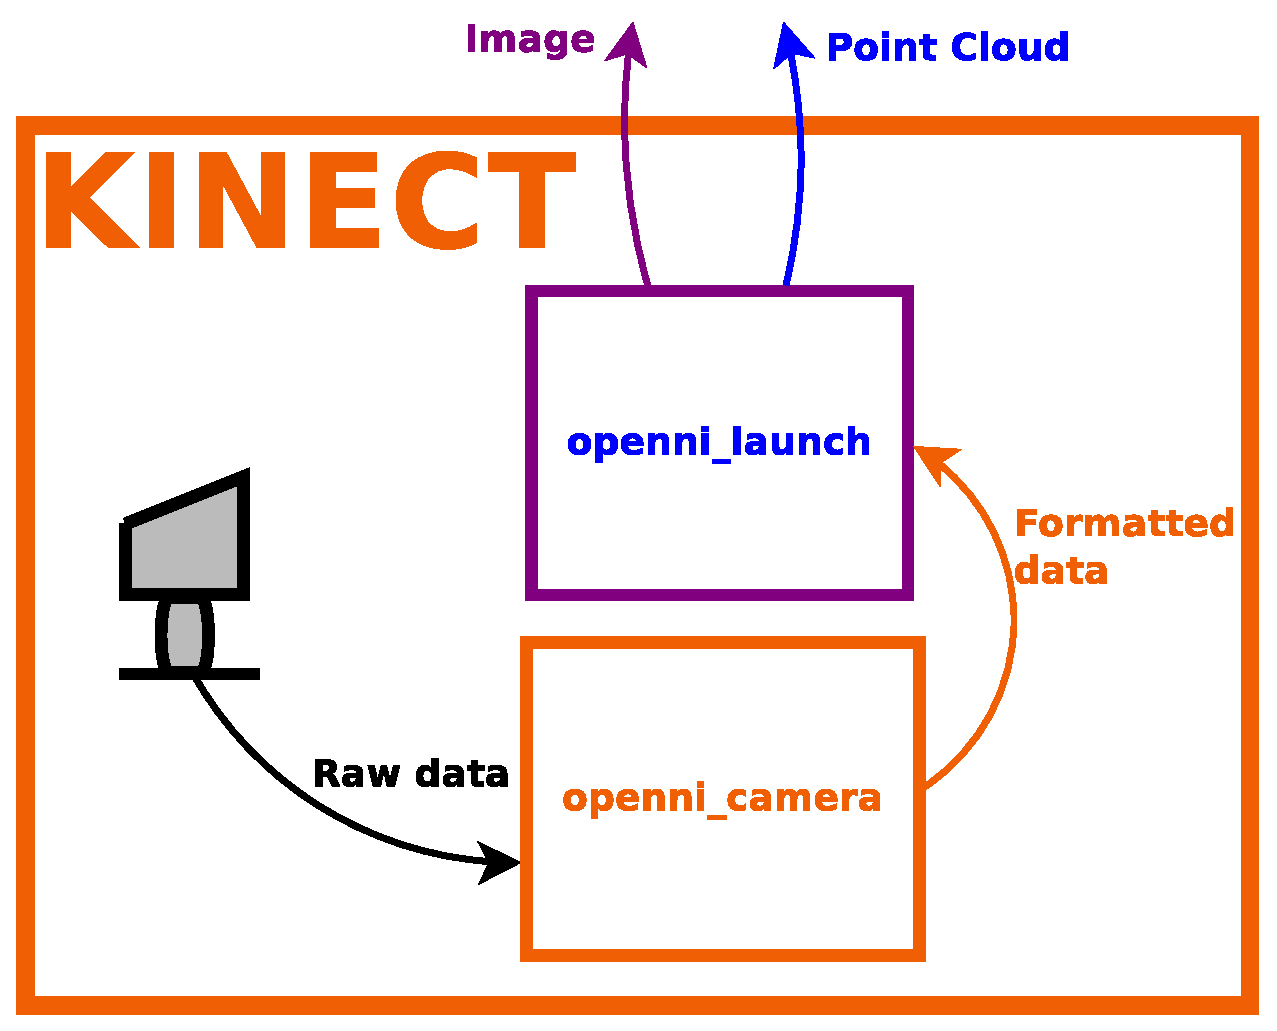
\includegraphics[width=0.5\linewidth]{img/diagrams/kinect_data.eps}
			\caption[Kinect data processing]{Kinect data processing using the openni ROS packages (openni\_camera and openni\_launch).}
			\label{diagram_kinect_data}
			\end{center}
		\end{figure}


\subsubsection{ROS package: openni\_launch}
\label{openni_launch}

This package provides useful transformations taking as input the openni\_camera topics. %and a launch file that executes nodelets with that information. 
It is composed of various nodes that can be executed using a launch file. 
Each node processes the raw input information from the driver into more useful data. 
This data may be a point cloud with color information or a disparity image for example. 
The output of the nodes is published into different topics. 
% The developed nodes described in section \ref{nodes} are subscribed to these topics in order to obtain the input point cloud and image. 
These topics are the input for the nodes that have been developed for this thesis.

\subsubsection{ROS package: pi\_tracker}
\label{pi_tracker}
This ROS package implements a joint tracker.
It is used within the system to determine the position and orientation of the user's joints. 
This task is performed by the skeleton tracker node.  
Figure \ref{diagram_skeleton} shows the Connectivity graph of this node. 
% In figure \ref{diagram_skeleton} it may be observed that the diagram presented in figure \ref{diagram_kinect_data} is simplified.  

		\begin{figure}[H]
			\begin{center}
			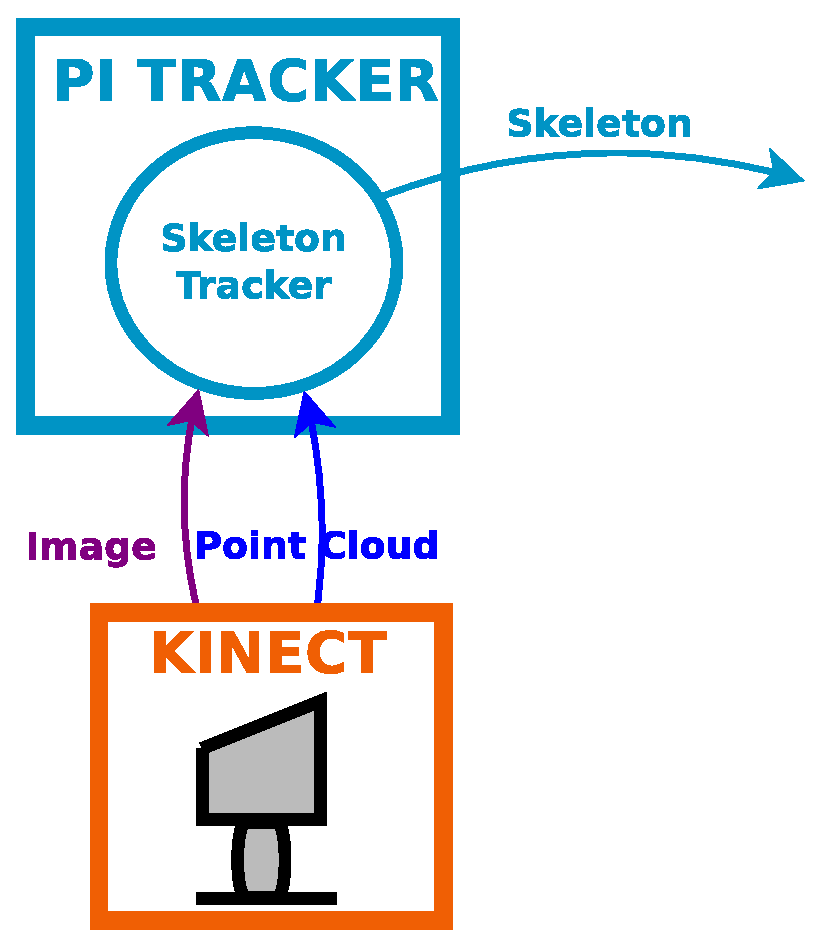
\includegraphics[width=0.3\linewidth]{img/diagrams/node_pi_tracker.eps}
			\caption[Skeleton Tracker I/O]{Connectivity graph of the Skeleton Tracker node.}
			\label{diagram_skeleton}
			\end{center}
		\end{figure}

It can be seen that the node takes as input the output data of the openni\_launch ROS package. 
The node outputs the Skeleton message in which the positions and orientations of the joints are represented. 



%\newpage
%%%%%%% SOFTWARE NODES %%%%%%
%\addcontentsline{toc}{subsection}{Software nodes}
\subsection{Description of the developed nodes}
\label{nodes}


The processing of the system is divided in nodes. 
Figure \ref{nodes_graph} shows the graph of the nodes that have been developed for the project.
% First the ones using the raw input data to the system and afterwards the ones that deliver the output of the system are described.
The circles represent the nodes. %Each circle is a node and the name inside them is the one being used in the software. 
The arrows show the communication between nodes. 
The names next to the nodes' interconnections are the messages interchanged.  % that those processes interchange. 
% The squares with the names serve as separators of the different packages that are being used. 
The square areas define the different ROS packages that have been used.
The square with the tile "OCULAR" separates the nodes developed in this thesis from third-party nodes. 
% All the nodes inside the square with the title "OCULAR" are the ones I developed. 
Sections \ref{converter} to \ref{last_node} present the processing performed by each node. 
\\


		\begin{figure}[H]
			\begin{center}
			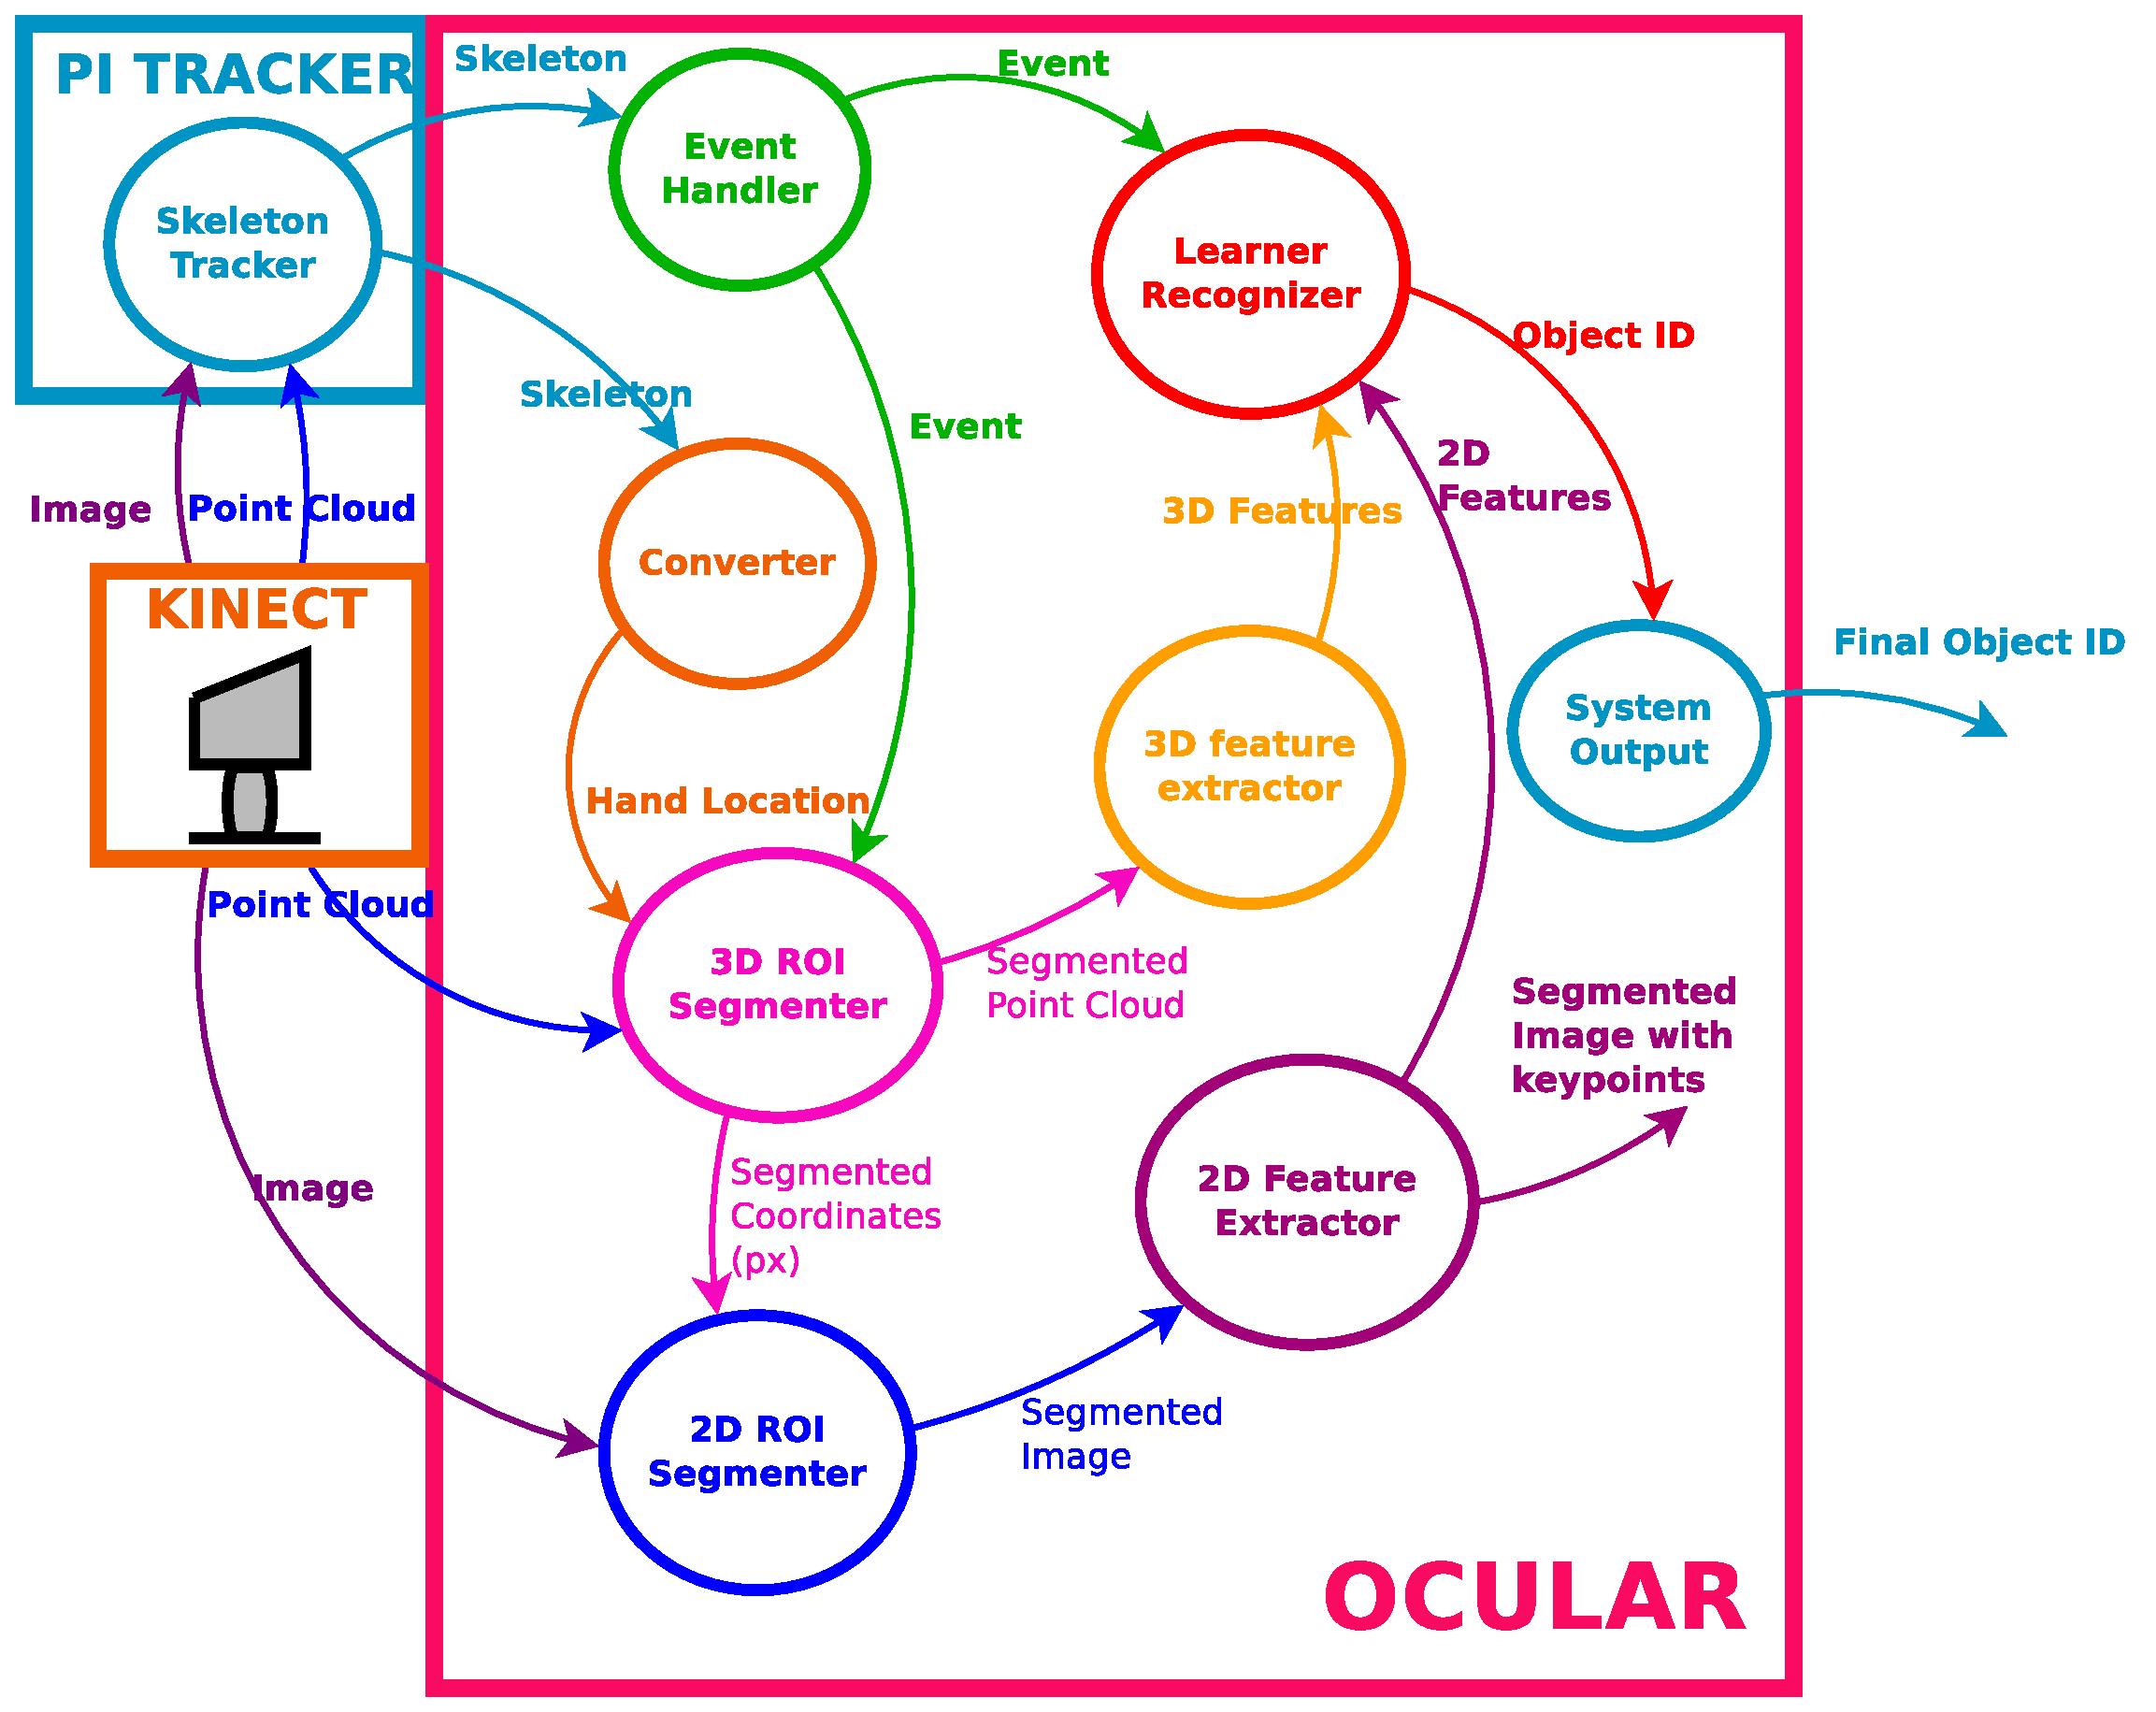
\includegraphics[width=\linewidth]{img/diagrams/nodes.eps}
			\caption[System nodes]{System nodes and their interaction.}
			\label{nodes_graph}
			\end{center}
		\end{figure}

%\newpage



%%\newpage


\subsubsection{Converter node}
		\label{converter}

	This node is the first step of the developed software, a translator to isolate the OCULAR package from third party packages. 
	It converts the input data containing the skeleton position to a custom message used through the rest of the code. 
	It allows to easily change the package from which the skeleton is obtained without affecting the whole system. 
	The converter node transforms the input data from the pi\_tracker package into the custom message used within the software. 
	It was only implemented a converter for the pi\_tracker package, but it could be easily developed a converter for other packages that retrieve the skeleton position. 
	Figure \ref{converter_graph} represents the Connectivity graph of the node. 
	The skeleton message enters the node and the custom message containing the hands location is the output. 

		\begin{figure}[H]
			\centering
			\includegraphics[width=0.5\linewidth]{img/diagrams/node_converter.png}
			\caption[Converter node I/O]{Connectivity graph of the Converter node.}		
			\label{converter_graph}
		\end{figure}

	% The information provided by that third-party code contains the position in the space of each joint of the body. 
	% The converter node takes only both hand's position. 
	The use case diagram of the node can be seen in figure \ref{uc_converter}. 
	Since it is a simple translator node, it has only three cases. 
	Receive the skeleton message is the first one. 
	The skeleton message is obtained from the third party package that tracks the user's skeleton.
	In this system, the package that tracks the skeleton is pi\_tracker (see section \ref{pi_tracker} for further information). 
	The second case is to select the hand's location from the input message. 
	This is the conversion step of the node, in which the information from the third-party package is parsed and the data relevant to the system's nodes is extracted. 
	Finally, the last case is to publish the location of the user's hands. 
	This is the output of the system, the custom message used within the system in which the hands location is specified. 
	\begin{figure}[H]
		\centering
		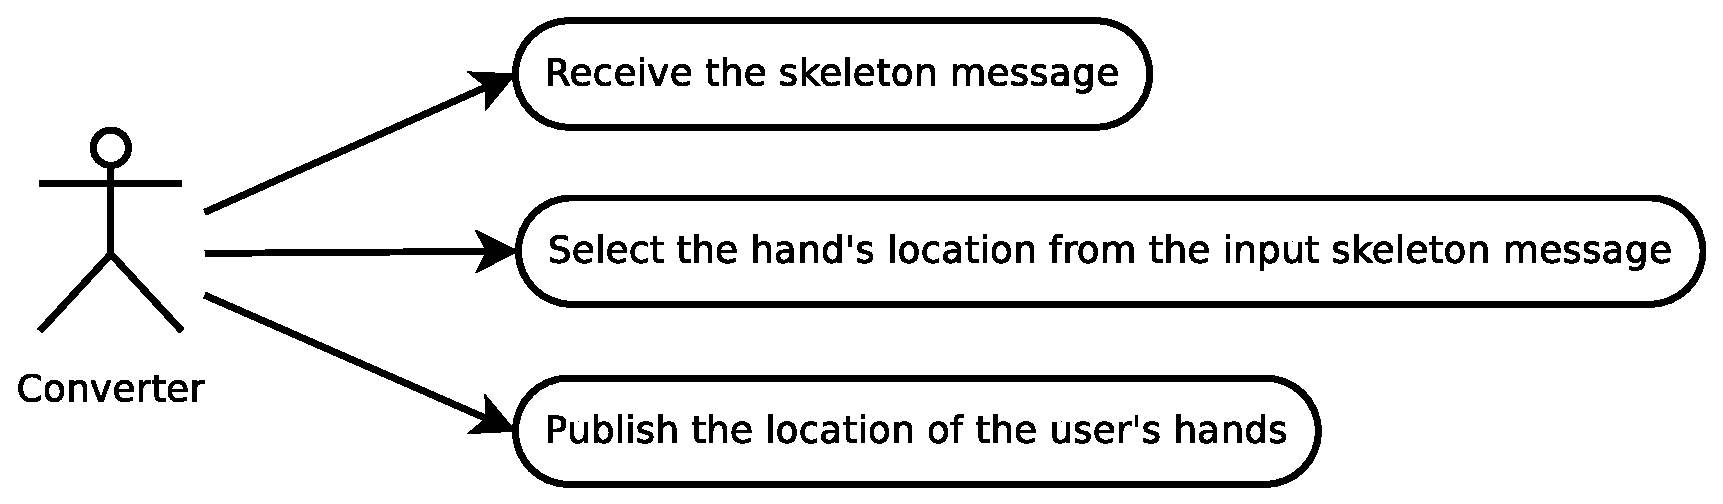
\includegraphics[scale=0.4]{img/diagrams/uc_converter.eps}
		\caption[Use case diagram converter node]{Use Case diagram of the converter node}
		\label{uc_converter}
	\end{figure}

	
	%%\newpage

\subsubsection{3D ROI Segmenter node}
	\label{roi_segmenter_3d}

	This node extracts the 3D Region Of Interest from the input point cloud. 
	This process is useful to eliminate useless information and hence reduce the size of the 3D data used by the system.  
	Having a smaller 3D data size also lowers the computing time of the following nodes that use this information. 
	Figure  \ref{node_roi3d} presents the Connectivity graph of the node. 
	The input of this node is the raw 3D information from the sensor and the hand's locations from the third-party package pi\_tracker, as well as the hand in which the user is holding the object. 

		\begin{figure}[H]
			\begin{center}
			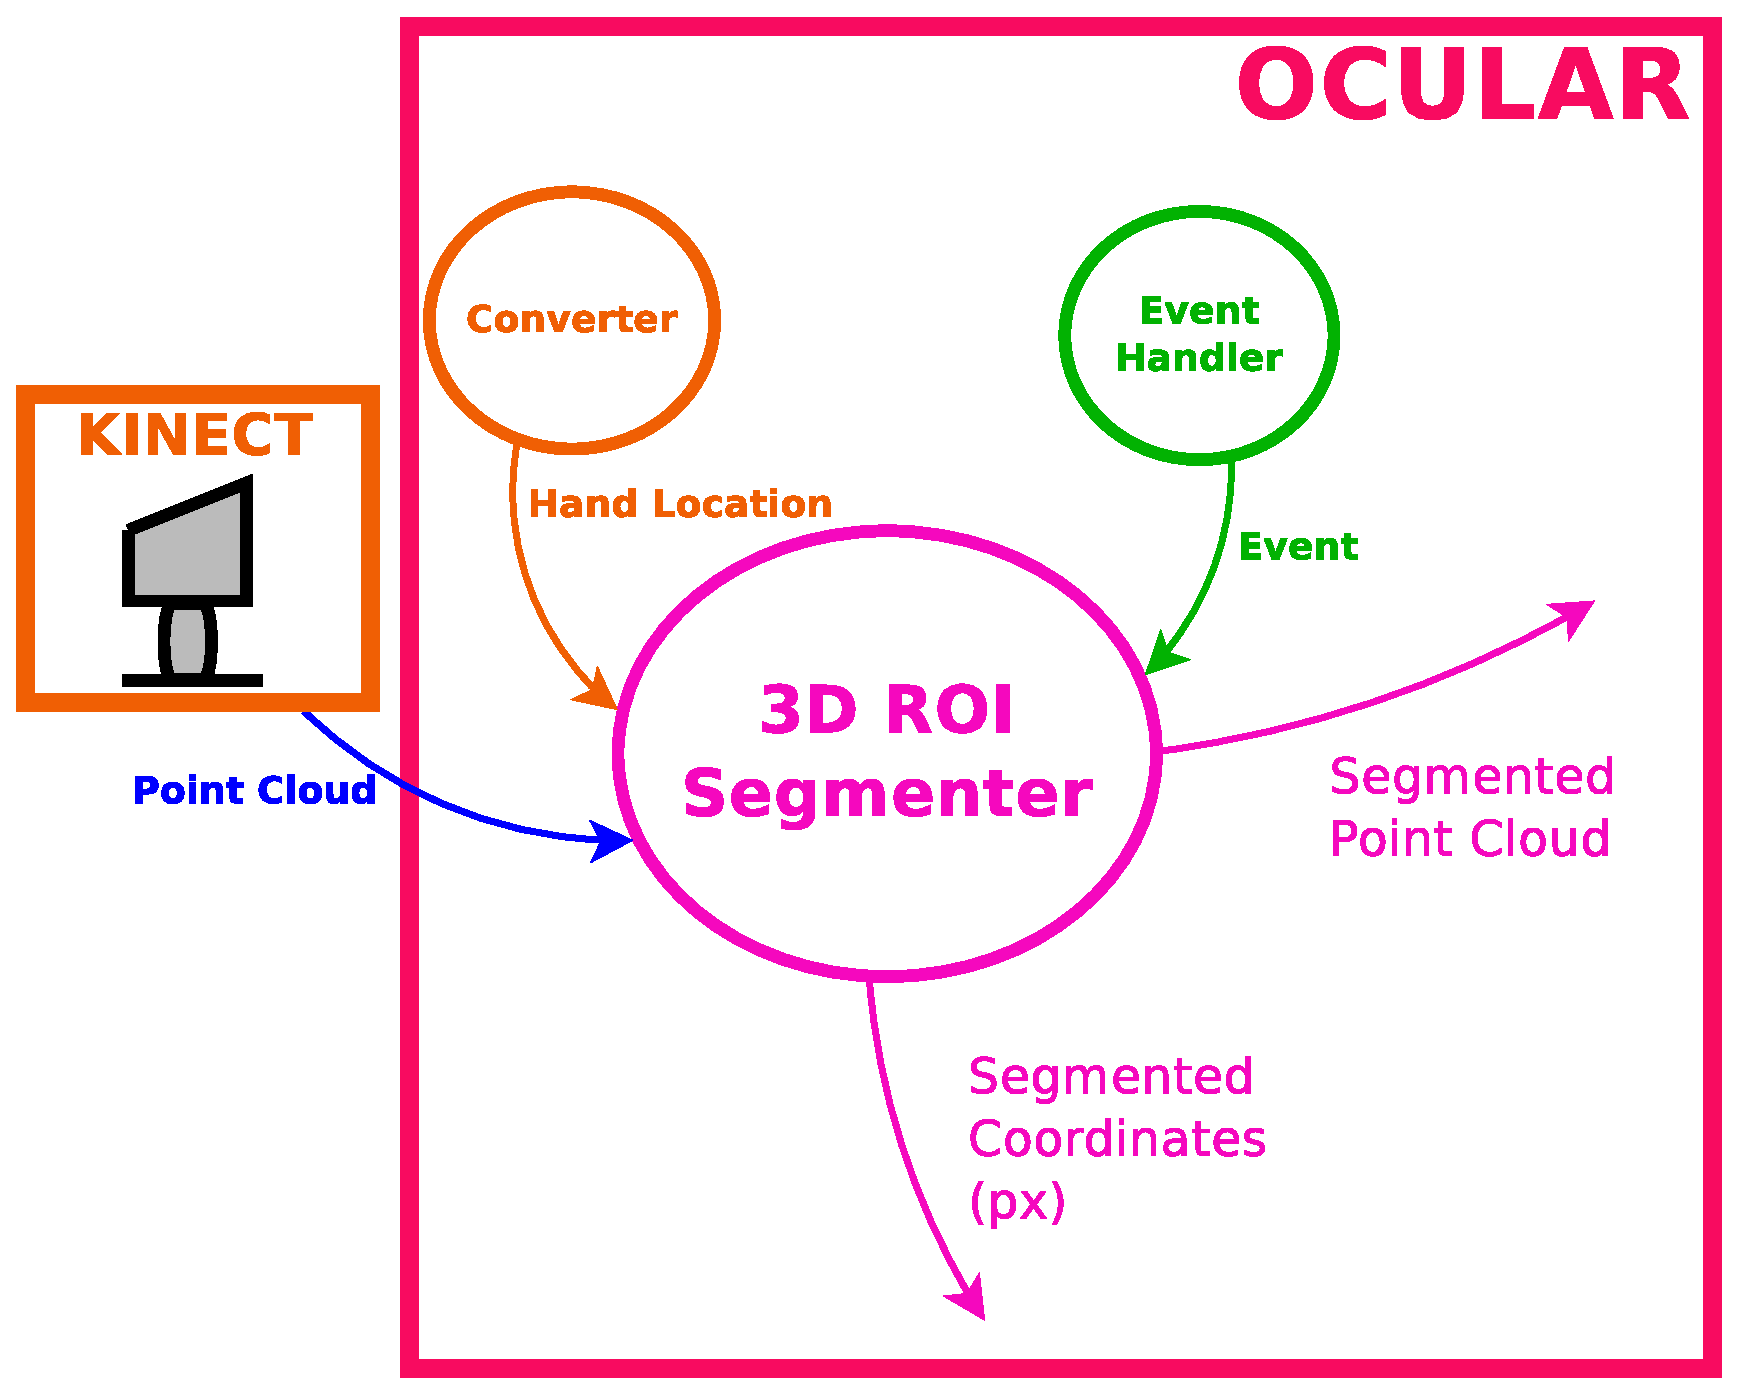
\includegraphics[width=0.5\linewidth]{img/diagrams/node_roi3d.eps}
			\caption[ROI segmenter 3D node I/O]{Connectivity graph of the ROI segmenter 3D node.}		
			\label{node_roi3d}
			\end{center}
		\end{figure}


	The system is used to detect in-hand objects. 
	Hence, the hand and the area around it conform the Region Of Interest of the software. 
	This is the reason why this node segments a prism around the selected hand's center from the input point cloud.
	\\

	The 3D ROI Segmenter node provides information to two different nodes: the 3D Feature Extractor (see section \ref{fe3d}) and the 2D ROI Segmenter node (see section \ref{roi_segmenter_2d}). 
	The segmented point cloud is passed to the 3D Feature Extractor and the segmented coordinates are shared with the 2D ROI Segmenter node. 
	This latter needs the values of the prism vertex coordinates in order to crop the input image. 
	Nevertheless, the coordinates in the 3D ROI Segmenter node are in world units and hence they need to be converted into pixels. 
	This step can be observed in Figure \ref{uc_roi3d}, which shows the use case diagram of the node. 
	% The prism vertex coordinates are transformed from world coordinates to pixels. 
	% To allow the ROI Segmenter 2D to perform the cropping of the input image using those pixel values. 
	% That information is the output of the node, together with the segmented point cloud. 
	

	\begin{figure}[H]
		\centering
	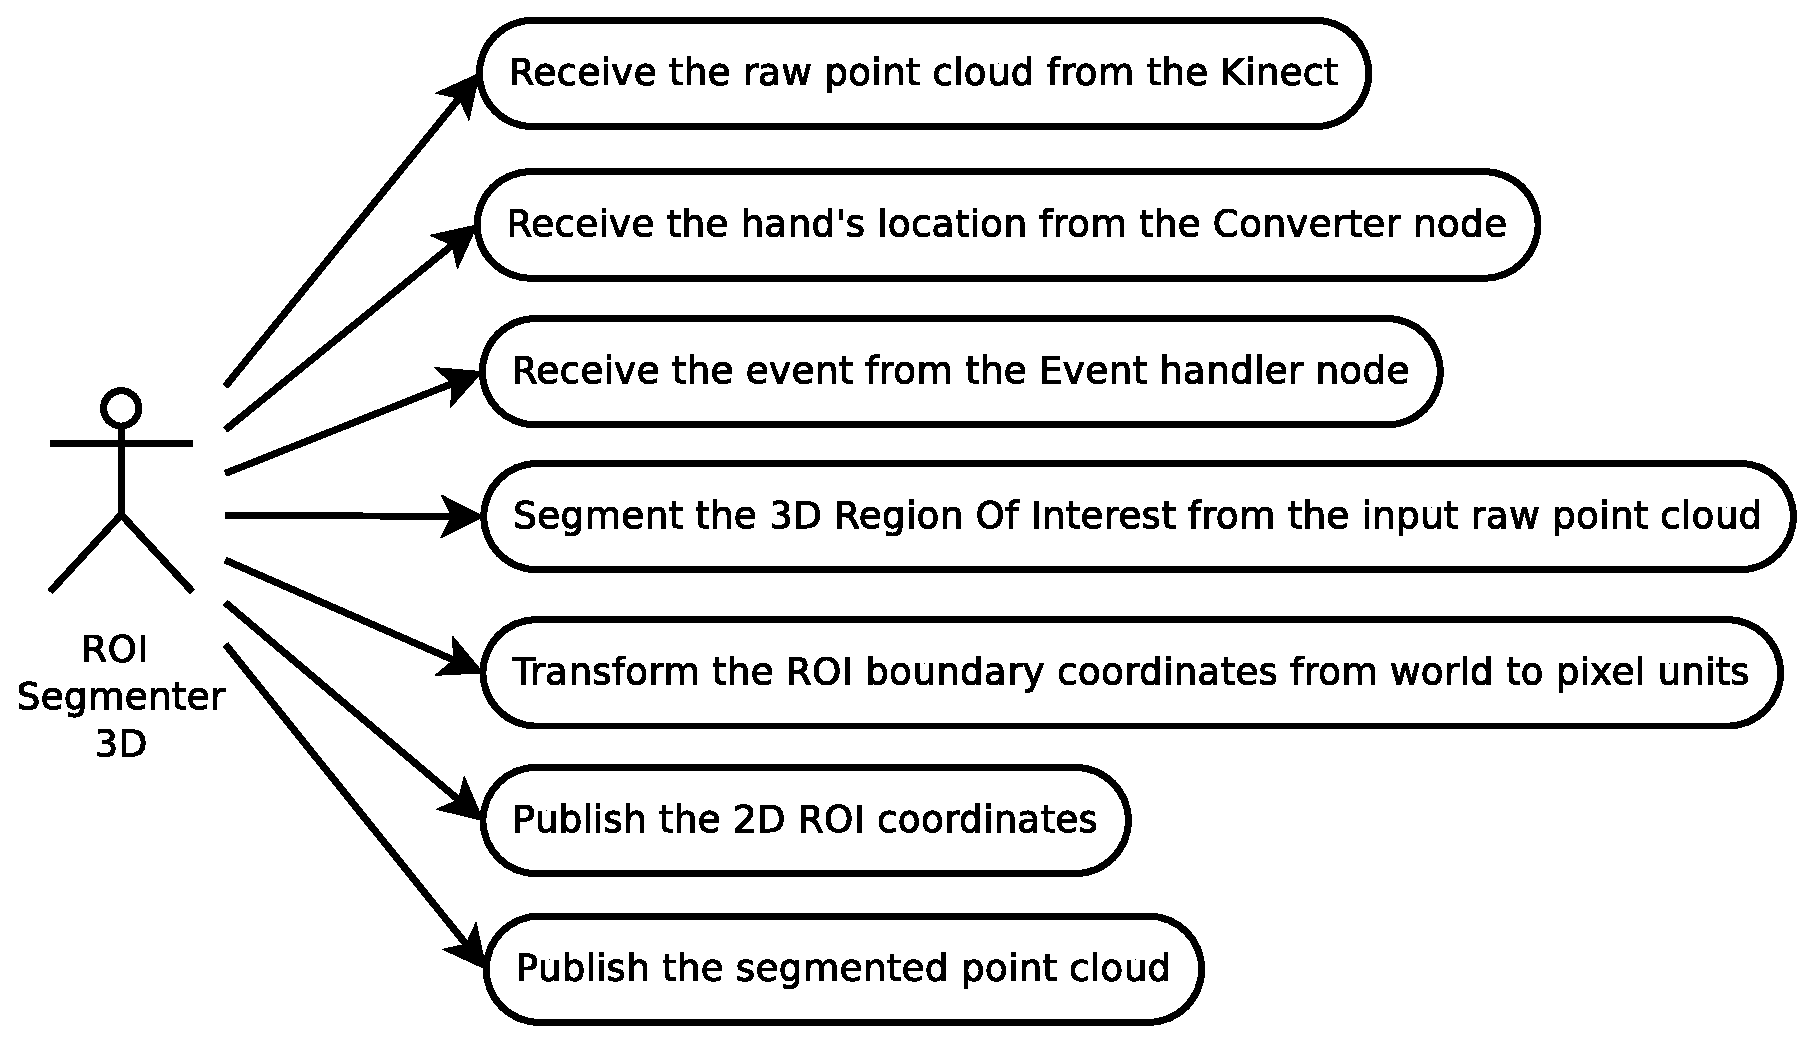
\includegraphics[scale=0.4]{img/diagrams/uc_roi_segmenter_3d.eps}
		\caption[Use case diagram ROI segmenter 3D node]{Use Case diagram of the ROI segmenter 3D node}
		\label{uc_roi3d}	
	\end{figure}
 
	In Figure \ref{uc_roi3d} the different cases of this node are shown. 
	Since this node is more complex than the previous Converter node (section \ref{converter}), there are more cases in which the program may be. 
	The first three present the reception of information: the raw point cloud from the kinect, the hand's location in the custom message used within the system from the converter node and the event from the event handler node. 
	This last piece of information is used to determine which hand is being used in the software. 
	Afterwards, the processing cases is presented: the segmentation of the 3D Region Of Interest from the input point cloud and the transformation of the boundary coordinates from world to pixel units. 
	Finally, the node publishes the segmented point cloud and the 2D ROI coordinates. 
%%\newpage

\subsubsection{2D ROI Segmenter node}
	\label{roi_segmenter_2d}
	
	%The present node takes as the input the raw 2D information from the RGB-D sensor and the hand's locations in pixels returned from the ROI segmenter 3D node. 
	Similarly to the previous node described in section \ref{roi_segmenter_3d}, this node is used to extract the Region Of Interest with the difference that this is segmented from the input 2D data, an image. 
	The reasons behind this operation are the same: eliminating the non-important part of the information allows to obtain a smaller data that reduces the computation times and also lowers the noise introduced to the system. 
	Figure \ref{node_roi2d} depicts the Connectivity graph of this node. 
	The raw 2D information and the hand location in pixels are inputs to the ROI Segmenter 2D node. 

		\begin{figure}[H]
			\begin{center}
			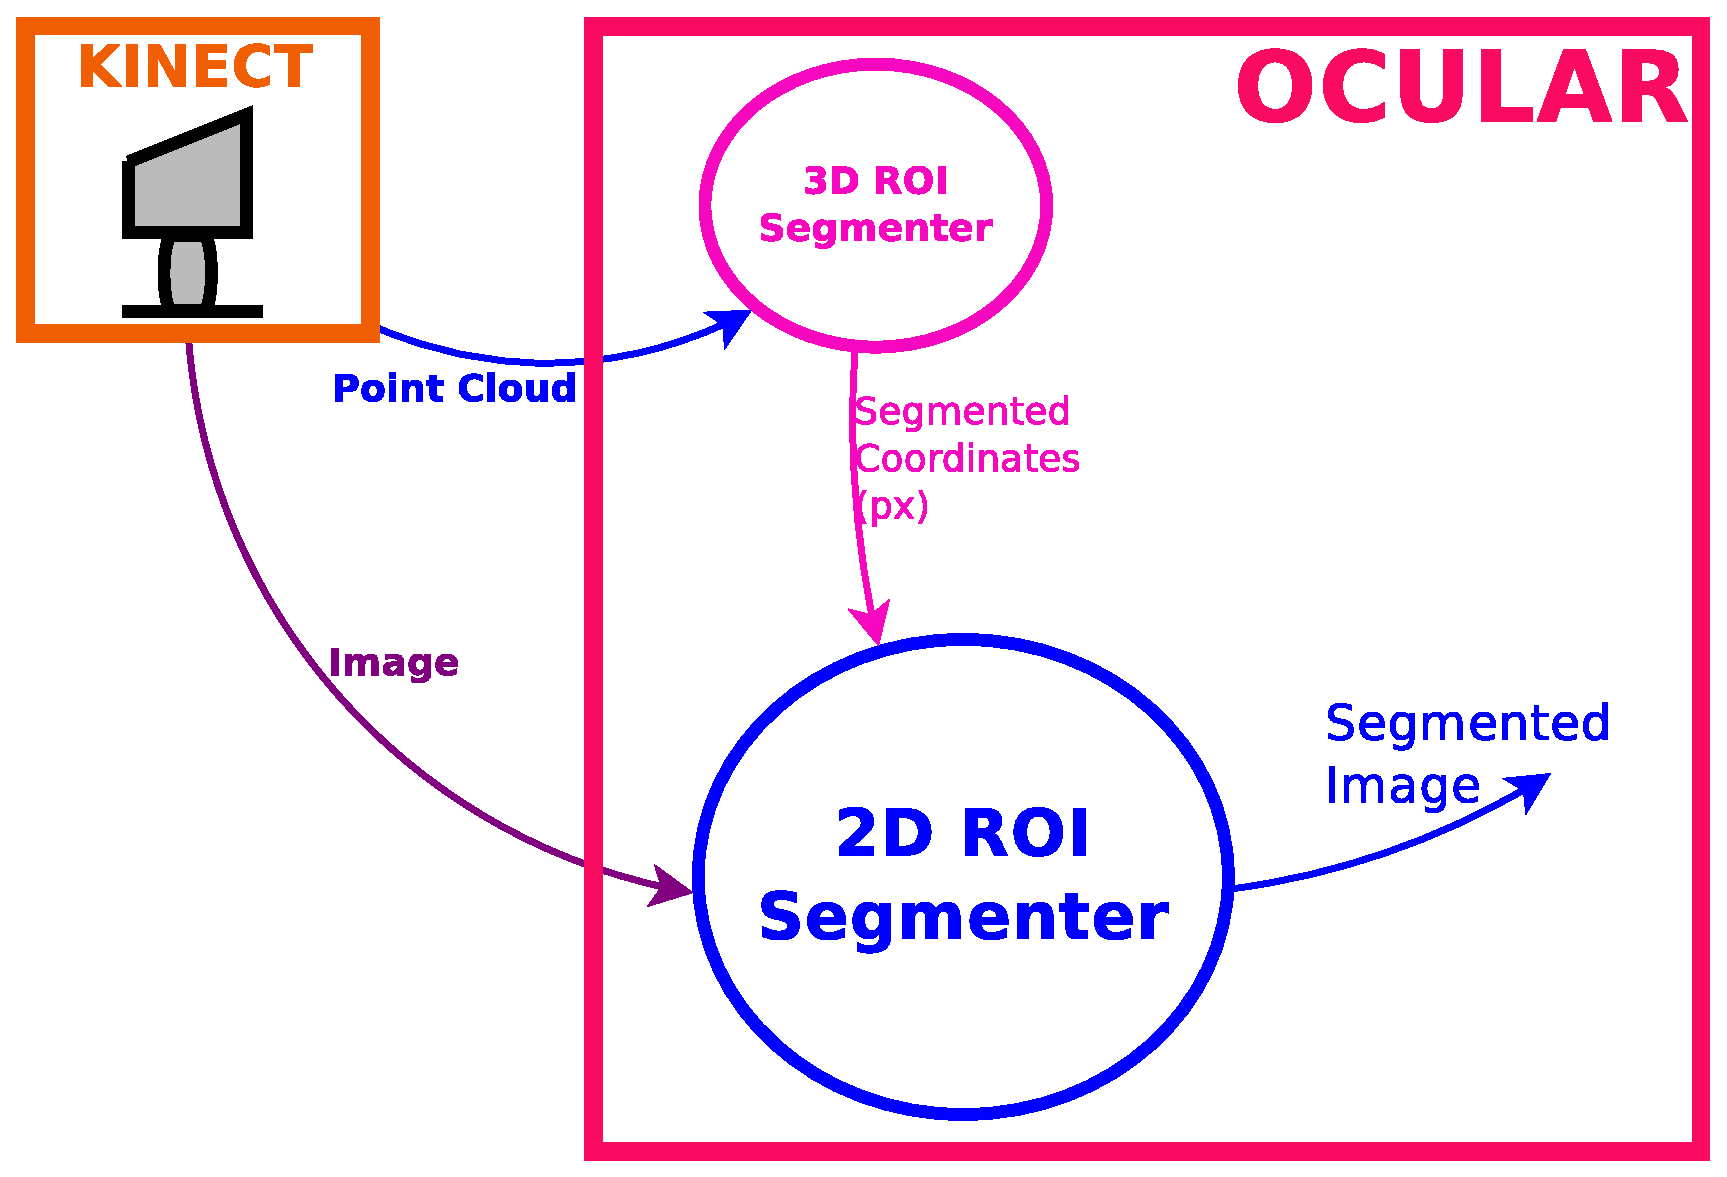
\includegraphics[width=0.5\linewidth]{img/diagrams/node_roi2d.eps}
			\caption[ROI segmenter 2D node I/O]{Connectivity graph of the ROI segmenter 2D node.}		
			\label{node_roi2d}
			\end{center}
		\end{figure}

	This node processes the information as follows: first, the ROI (Region Of Interest) is cropped taking a square section around the center of the hand. 
	The size of the square is fixed because the difference in the scale in negligible in the operating range of the system (1.5m to 2.5m). 
	This range is determined by the skeleton tracker node and also by the low resolution of the RGB-D sensor. 
	The skeleton tracker node operates correctly in that range. 
	If the person is located closer to the kinect, the node does not recognize the skeleton. 
	If the user is outside the range, it is considered a background object and hence the node does not track his skeleton. 
	%Since due to the RGB-D sensor's current resolutions the user must remain at a fixed distance from the sensor, the difference in the scale due to the distance is negligible and hence the size can be fixed. 
	\\
	\begin{figure}[H]
		\centering
			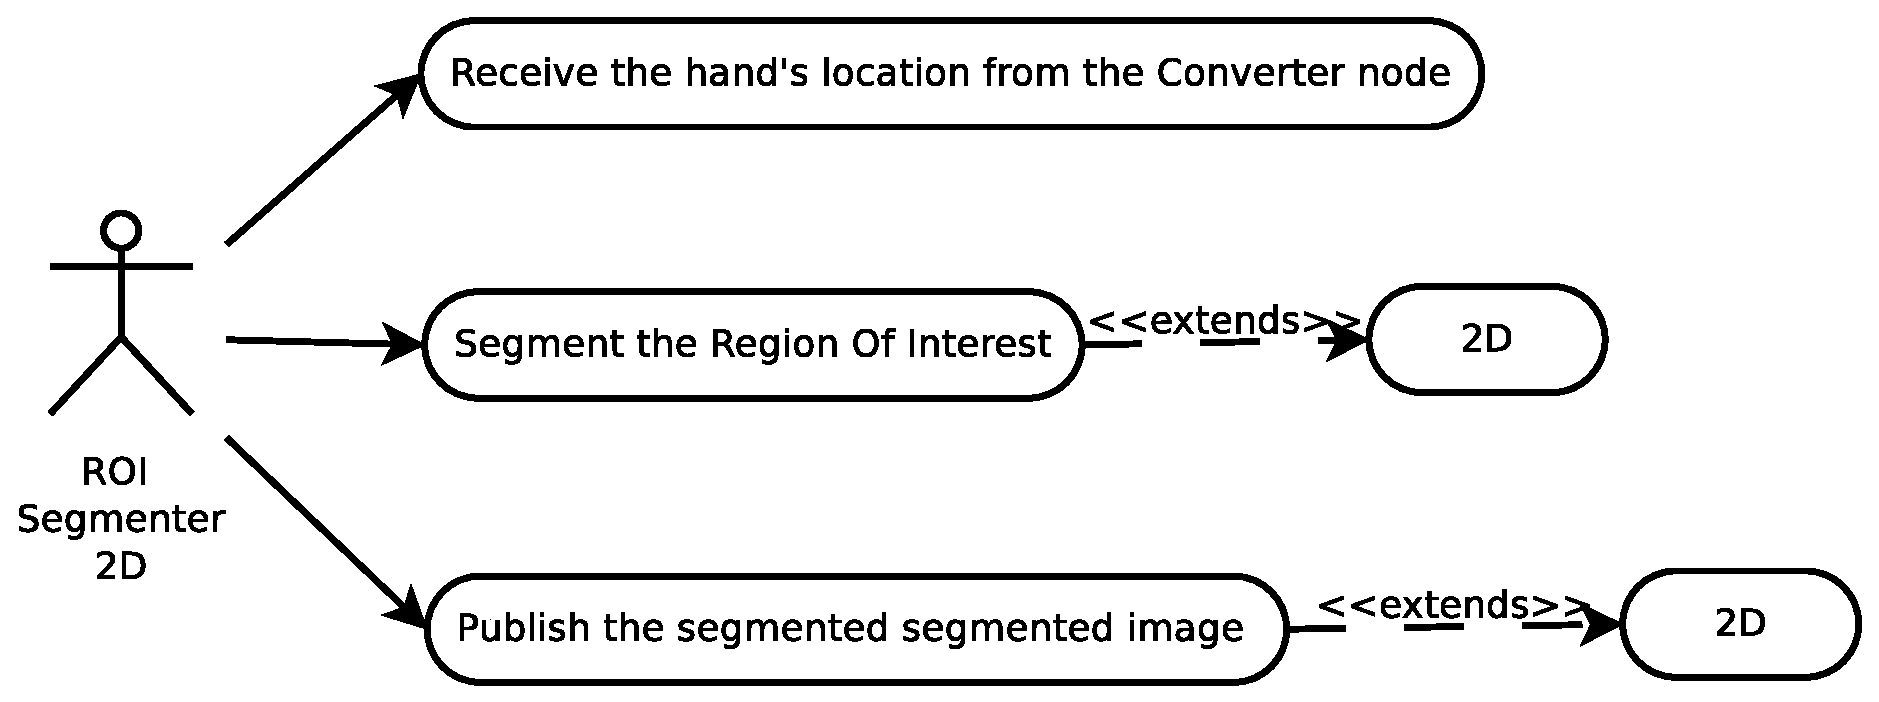
\includegraphics[scale=0.4]{img/diagrams/uc_roi_segmenter_2d.eps}
			\caption[Use case diagram ROI segmenter 2D node]{Use Case diagram of the ROI segmenter 2D node}
		\label{uc_roi2d}
	\end{figure}

	In figure \ref{uc_roi2d} the use case diagram of the node can be observed.
	The first two cases show the reception of information from other nodes such as the 2D ROI location from the 3D ROI Segmenter node, the raw image from the Kinect. 
	Then, the processing case is presented which is the segmentation or extraction of the 2D Region Of Interest. 
	Finally, the last case involves the publishing of that segmented information. 
%%\newpage

\subsubsection{2D Feature Extractor node}
\label{fe2d}
	This node is used to obtain the descriptors or characteristics from the segmented 2D information. 
	These features are used in later nodes to match two objects and determine whether they are the same one or not. 
	The 2D Feature Extractor node is hence the last part of the 2D data processing in the system. 
	% This node takes as an input the segmented 2D ROI from the previous nodes and extracts the features. 
	Figure \ref{node_fe2d} shows the Connectivity graph of the node. 

		\begin{figure}[H]
			\begin{center}
			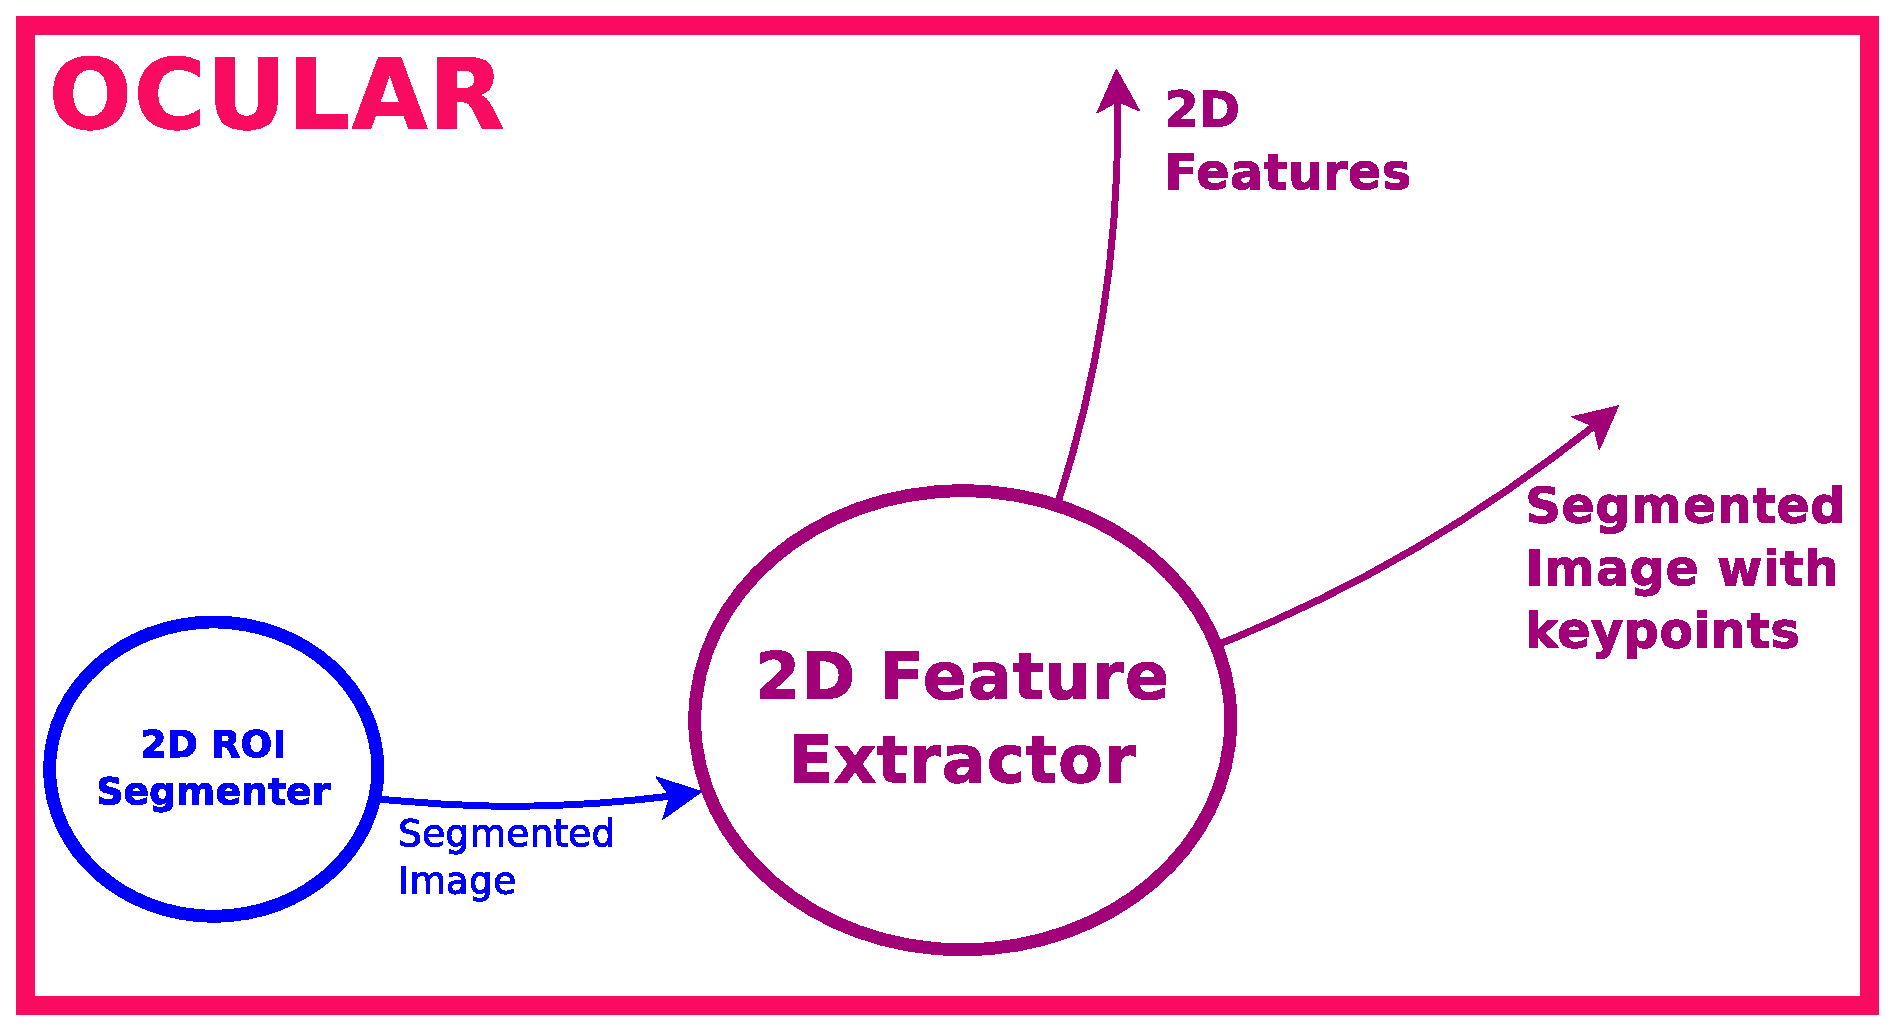
\includegraphics[width=0.5\linewidth]{img/diagrams/node_fe2d.eps}
			\caption[Feature Extractor 2D node I/O]{Connectivity graph of the Feature Extractor 2D node.}		
			\label{node_fe2d}
			\end{center}
		\end{figure}

	There are two output messages of this node, the segmented images with keypoints and the 2D ORB descriptors matrix. 
	This matrix is used in the rest of the system. 
	The segmented image with the keypoints drawn on it is outputted for debugging and development reasons. 
	\\

	Figure  \ref{uc_fe2d} represents the use case diagram of this node. 
	The first case shows the reception of the segmented image. 
	The two cases in the middle reflect the extraction of 2D features and the saving of those features to a file. 
	This last operation is only performed when the system is shut down to avoid a lag in the software in runtime. 
	Finally, the last case contains the publishing of the 2D features, which is used by the learner-recognizer node (see section \ref{learner_recognizer}) and the segmented image with keypoints, which is only used for debugging and developing. 
	\begin{figure}[H]
		\centering
			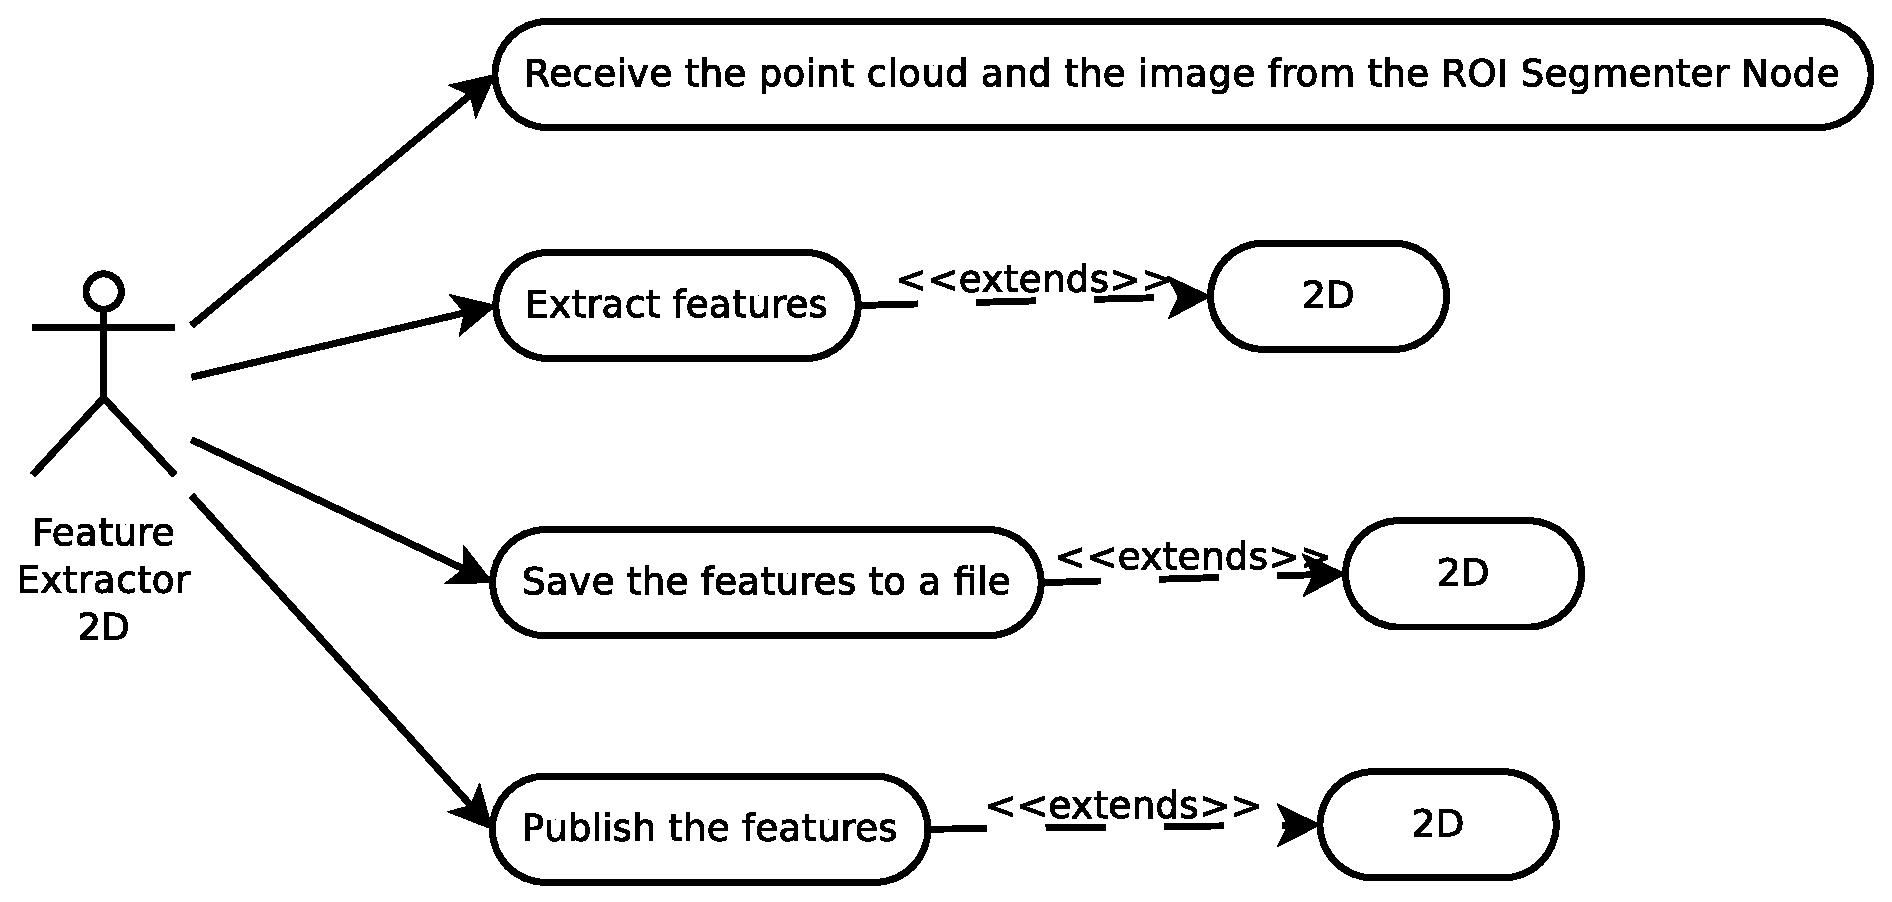
\includegraphics[scale=0.4]{img/diagrams/uc_feature_extractor_2d.eps}
			\caption[Use case diagram Feature Extractor 2D node]{Use Case diagram of the Feature Extractor 2D node}
		\label{uc_fe2d}
	\end{figure}

%%\newpage

\subsubsection{3D Feature Extractor node}
\label{fe3d}
	This node is used to extract the 3D features or descriptors from the segmented point cloud. 
	Those features are stored in a matrix, which is used to compare the data from different objects. 
	This comparison is performed in the Learner-Recognizer node (see section \ref{learner_recognizer}).
	Figure \ref{node_fe3d} shows that the input of this node is the segmented point cloud from the ROI Segmenter 3D node (see section \ref{roi_segmenter_3d}). The descriptors are extracted from this information and are published in the output topic. 
	\\
		\begin{figure}[H]
			\begin{center}
			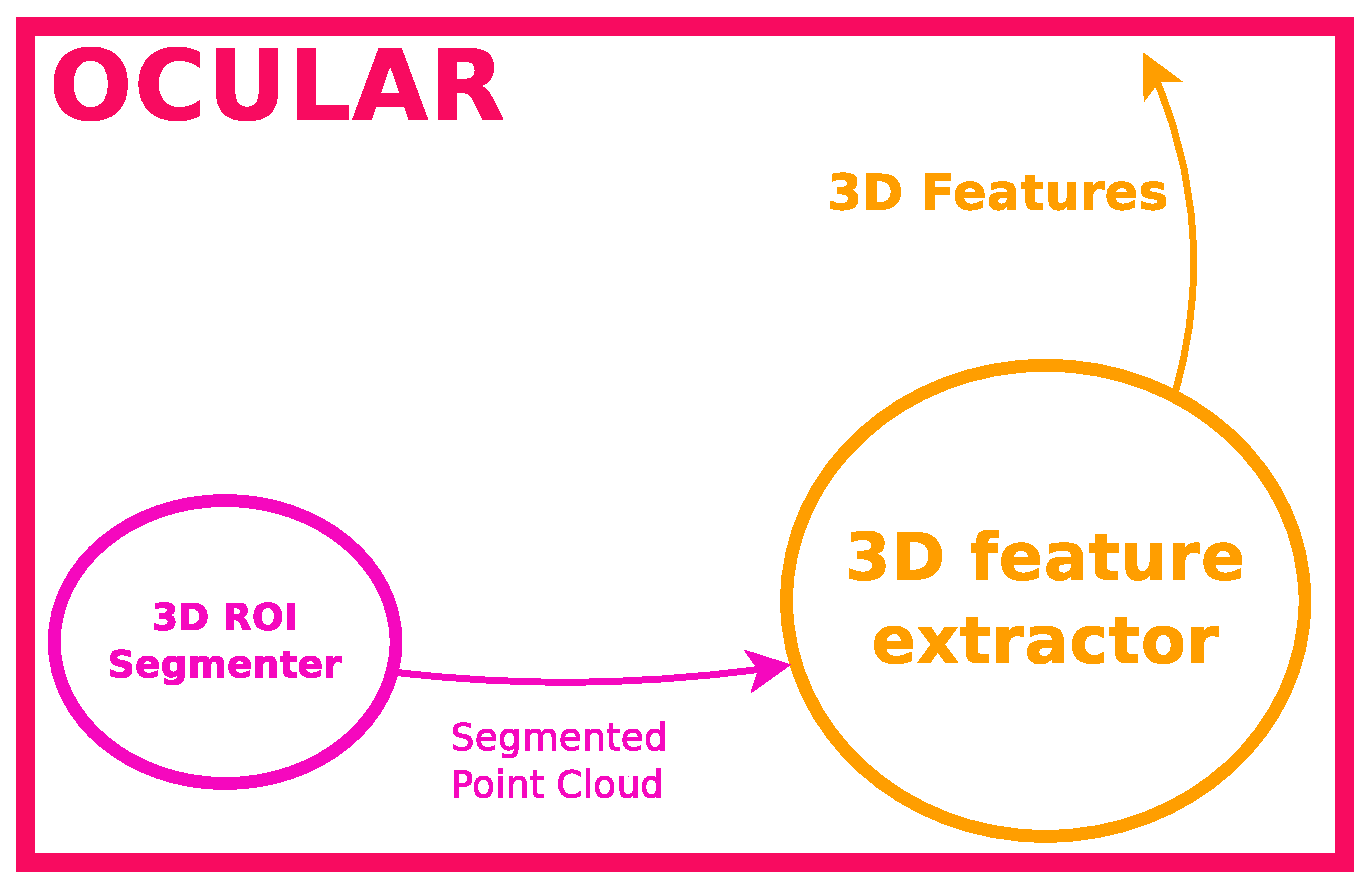
\includegraphics[width=0.5\linewidth]{img/diagrams/node_fe3d.eps}
			\caption[Feature Extractor 3D node I/O]{Connectivity graph of the Feature Extractor 3D node.}		
			\label{node_fe3d}
			\end{center}
		\end{figure}

	Figure \ref{uc_fe3d} shows the use case diagram of the node, which is very similar to figure \ref{uc_fe2d} from the 2D Feature Extractor node (section \ref{fe2d}). 
	The first case presents the acquisition of the segmented point cloud. 
	The two following cases are the processing of the node: the extraction of 3D features and the saving of this features to files in the system's shut down. 
	The final case involves the publishing of these 3D features. 

	\begin{figure}[H]
		\centering
			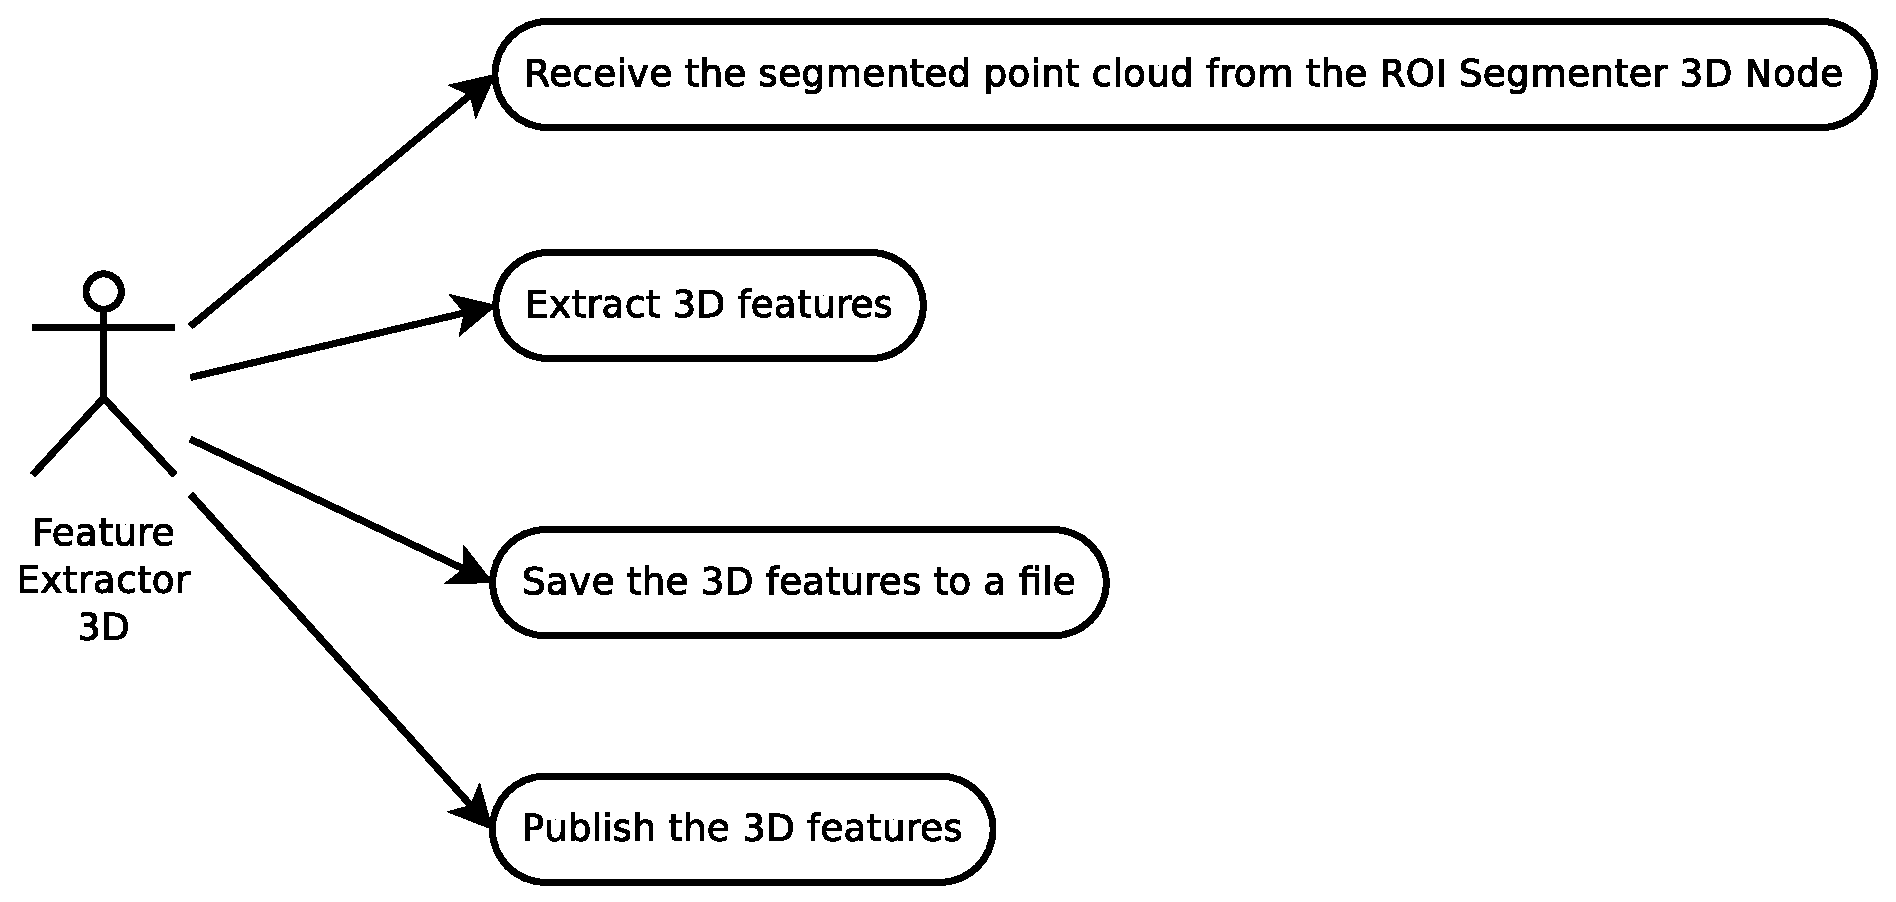
\includegraphics[scale=0.4]{img/diagrams/uc_feature_extractor_3d.eps}
			\caption[Use case diagram Feature Extractor 3D node]{Use Case diagram of the Feature Extractor 3D node}
		\label{uc_fe3d}
	\end{figure}

%%\newpage

\subsubsection{Event Handler node}
\label{event_handler}
	The system is intended to be running in a robot. 
	This implies that there are no devices such as a mouse or a keyboard to interact with it. 
	Hence, an Event Handler node is needed to allow the human-machine interaction using gestures. 
	There are two gestures or poses that the system detects. 
	If the user has the arm stretched towards the RGB-D (Red, Green, Blue and Depth) sensor the event recognized is \textit{"Learn"}. 
	If the arm is located near the user's body, the event is \textit{"Recognize"}. 
	The first event triggers the learning cycle described in section \ref{learning_mode}. 
	The second event is the default of the system and enables the recognition of the in-hand objects. 
	\\

	This node also selects the hand that is being used in the software. 
	The system is able to work with one hand at a time. 
	The user's pose to use the software is having the hand that has no object near the body and the one holding the object shigher. 
	% As it was previously stated, in order to interact with the software some gestures were defined. 
	% This is the module that detects those gestures and switches the event message accordingly to the corresponding event. 
	% This is the node responsible of detecting the different events that the user triggers. 
	\\

	Figure \ref{node_event} shows the connectivity graph of the node. 
	Event Handler receives its input from the pi\_tracker package and outputs the event message to the rest of the system. 

		\begin{figure}[H]
			\centering
			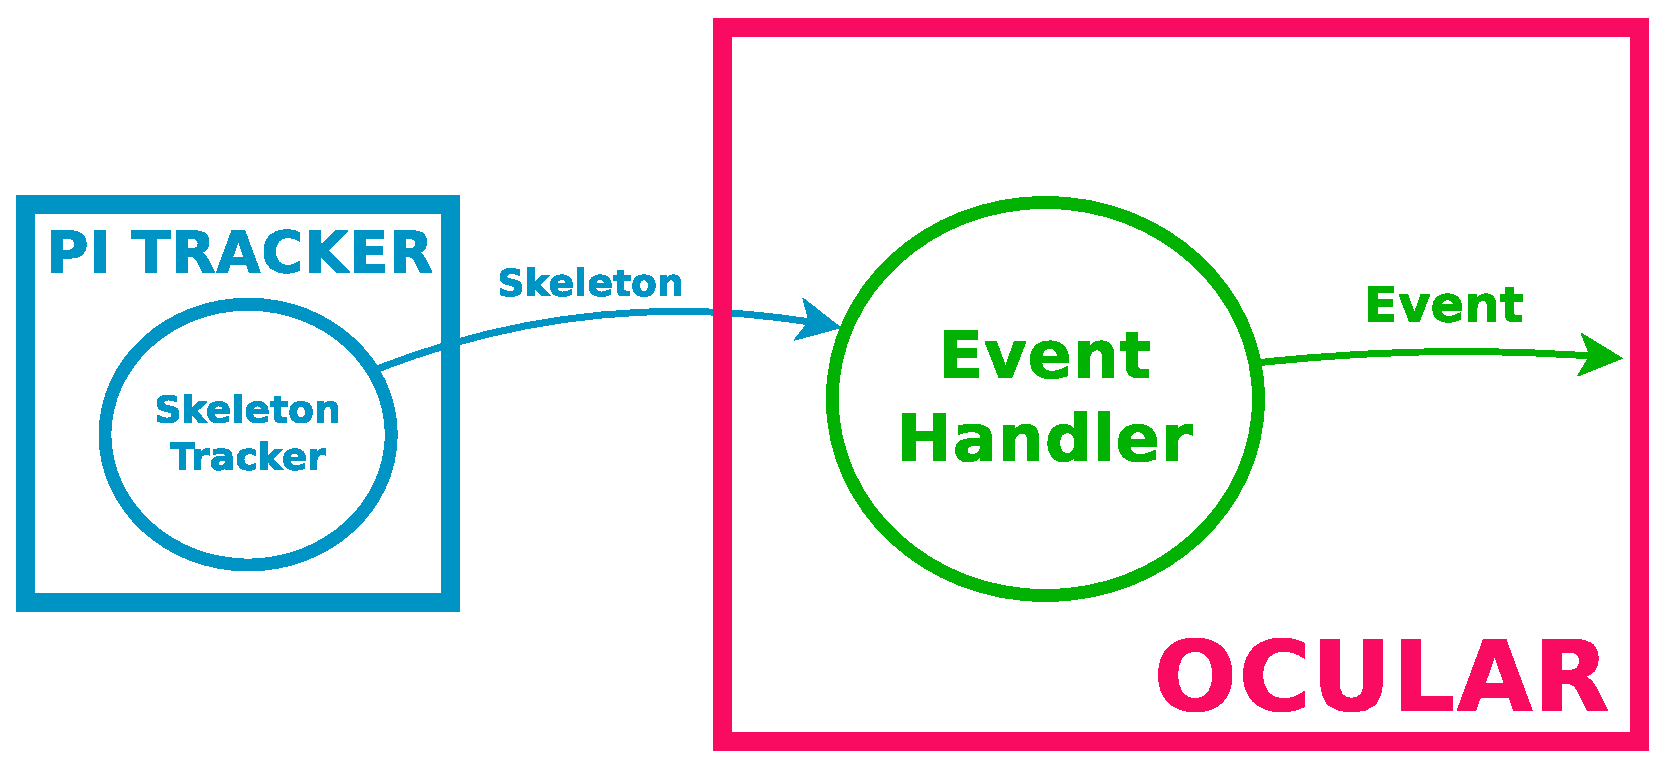
\includegraphics[width=0.5\linewidth]{img/diagrams/node_event.eps}
			\caption[Event Handler 3D node I/O]{Connectivity graph of the Event Handler node.}		
			\label{node_event}
		\end{figure}

	The input of the system is the skeleton message that is obtained from the third-party package pi\_tracker. This message contains the information of all the joints of the user. The information is screened to detect the height at which each hand is located. The one that is the highest is the one being used in the software. Afterwards, the distance between the body and the chosen hand is computed. When that distance is similar to the distance of the user's arm, the event triggered is "learn". If, otherwise, the hand is located close to the body, the event that is published to the output topic is "recognize". 
	The distance that triggers the modes is proportional to the distance between the user and the RGB-D sensor in order to obtain a range of use of the software higher. 
	\\

	Figure \ref{uc_event} is a diagram with the use case of the node. 
	The first case shows the input of the information about the relative hand's position from the pi\_tracker node. 
	Afterwards, the event being triggered is decided and finally published. 
	The information of the events is used in the Learner-Recognizer node (section \ref{learner_recognizer}).
	\begin{figure}[H]
		\centering
			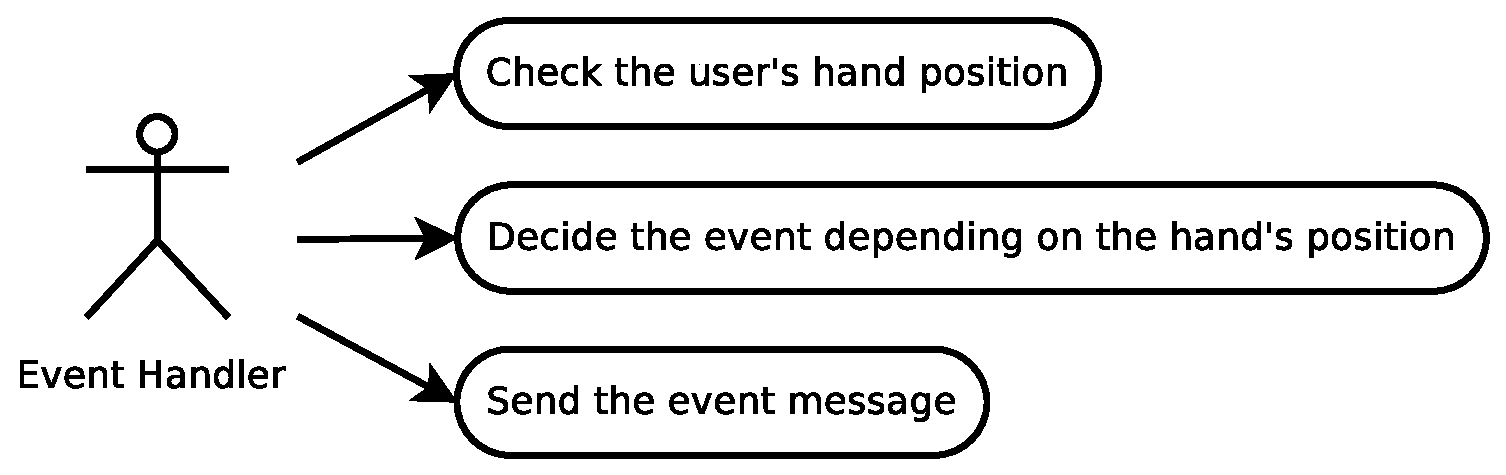
\includegraphics[scale=0.4]{img/diagrams/uc_event_handler.eps}
			\caption[Use case diagram Event Handler node]{Use Case diagram of the Event Handler node}
		\label{uc_event}
	\end{figure}

%%\newpage

\subsubsection{Learner-Recognizer node}
\label{learner_recognizer}
	This node implements the state machine of the system. 
	It is needed to switch the mode of the software accordingly with the event being triggered by the user.  
	% This node implements the state machine depending on the events recognized by the event handler node.
	If the event received is "Learn", the learning sequence starts. If the event is "Recognize", the recognize sequence is triggered. 
	These events are detected by the Event Handler node, described in section \ref{event_handler}
	\\

		\begin{figure}[H]
			\begin{center}
			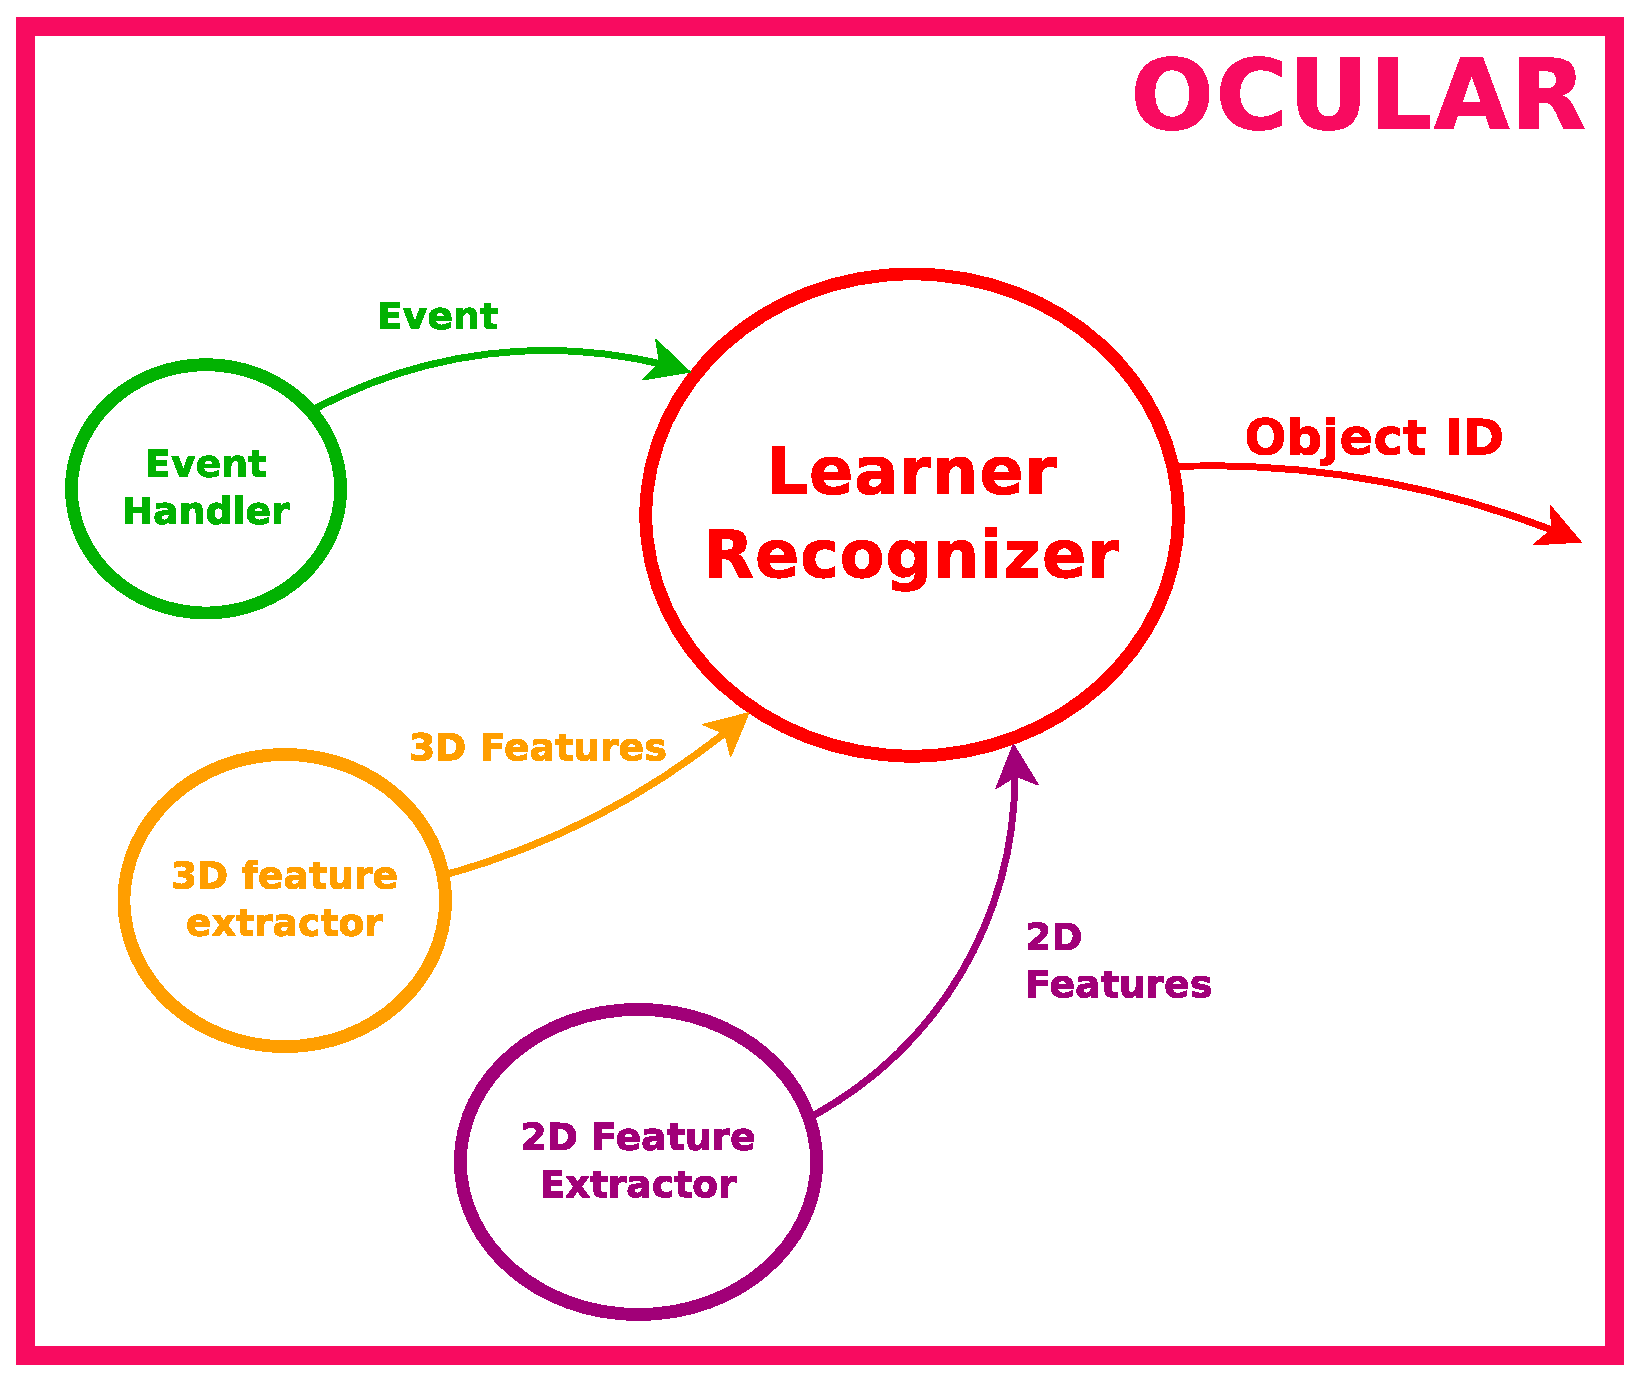
\includegraphics[width=0.5\linewidth]{img/diagrams/node_lr.eps}
			\caption[Learner-Recognizer node I/O]{Connectivity graph of the Learner-Recognizer node.}		
			\end{center}
						\label{node_lr}

		\end{figure}

	The learn sequence consists in obtaining and storing the features both 2D and 3D and waiting a second allowing the user to move the object to capture a new view of it. 
	The dataset extracted is saved to a folder when the software is closed, to prevent possible lags in the runtime of the program. 
	Each view is saved separately. 
	This node loads the files that are still in the saving folder when the program is restarted. 
	\\

	The recognition sequence compares the newly obtained features both 2D and 3D with the ones that are stored in the dataset. 
	Afterwards, the result of the recognition for both types of descriptors are published in the output topic. 
	Figure \ref{uc_learner_recognizer} presents the use case diagram of the node. 

	\begin{figure}[H]
		\centering
			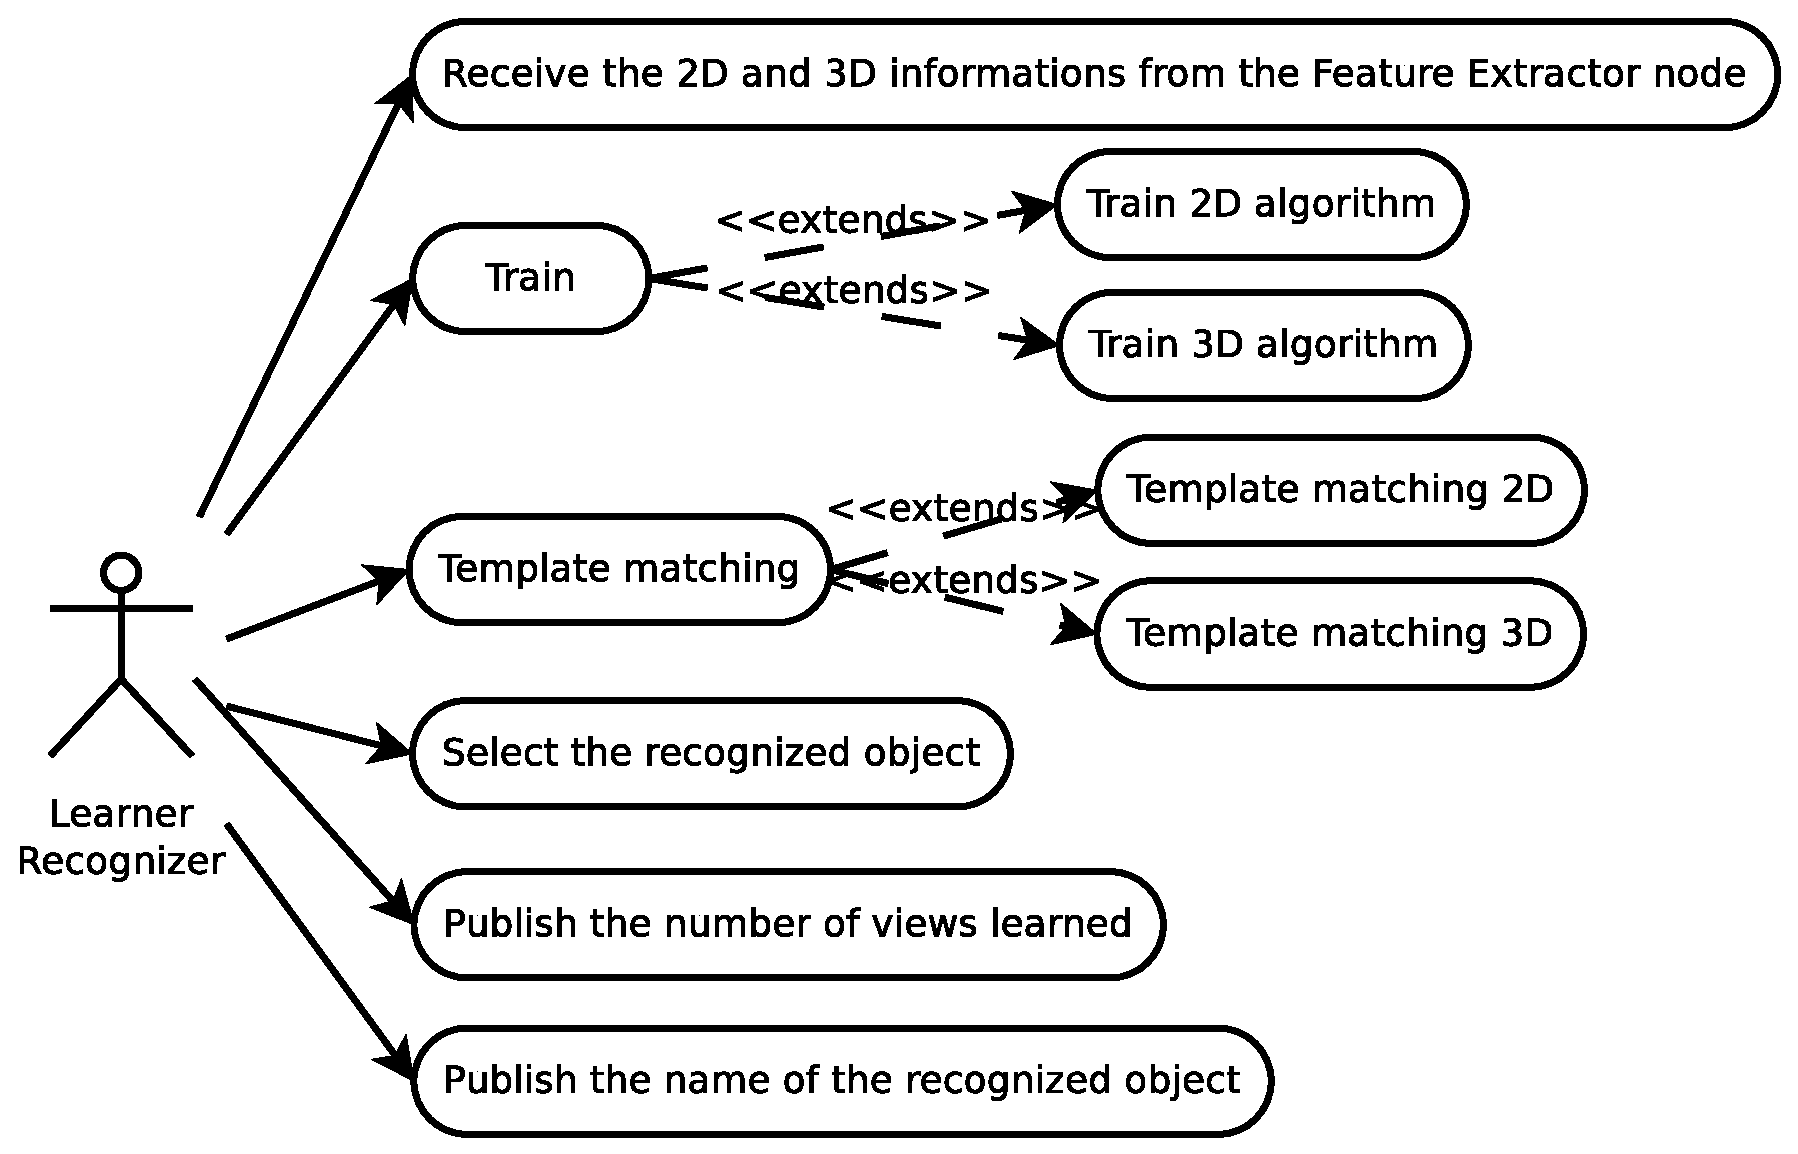
\includegraphics[scale=0.4]{img/diagrams/uc_learner_recognizer.eps}
			\caption[Use case diagram Learner-Recognizer node]{Use Case diagram of the Learner-Recognizer node}
			\label{uc_learner_recognizer}
	\end{figure}

	The first two cases are the data acquisition. 
	That data is the event that the user has triggered and the 2D and 3D features from both Feature Extractor nodes (sections \ref{fe2d} and \ref{fe3d}).
	Afterwards, the train case is shown which is performed for both 2D and 3D descriptors.
	In the middle, the case that implements the state machine is presented: the switching between the training and the recognizing modes. 
	Then, the template matching case appears that is also performed on 2D and 3D. 
	In it, the descriptors extracted from the current frame are compared to those previously obtained.
	The next case is the selection of the recognized object. 
	The information is obtained for the 2D and 3D information separately. 
	This information is then published at a rate of approximately thirty messages per second. 

%%\newpage


\subsubsection{System Output node}
\label{last_node}
	The output of the Learner-Recognizer node described in section \ref{learner_recognizer} is the predicted object. 
	This prediction is very noisy due to different factors such as sudden changes in the illumination of the room. 
	In order to reduce the noise effect in the system, it was decided to introduce the System Output node. 
	This nodes is a low-pass filter, which means that it eliminates those results that has a high frequency. 
	This task is performed using a buffer to store a certain amount of predictions and then managing the stored data. 
	% This nodes implements a buffer and a decision algorithm. 
	\\

	The input of the node is the object ID message from the Learner-Recognizer process as can be seen in figure \ref{node_output}.
	The node stores thirty values of instantaneous object estimations. 
	Since the Kinect runs at 30 frames per second, approximately each second a new final object estimation is outputted. 
	% The output of the node is the final object ID. 


		\begin{figure}[H]
			\begin{center}
			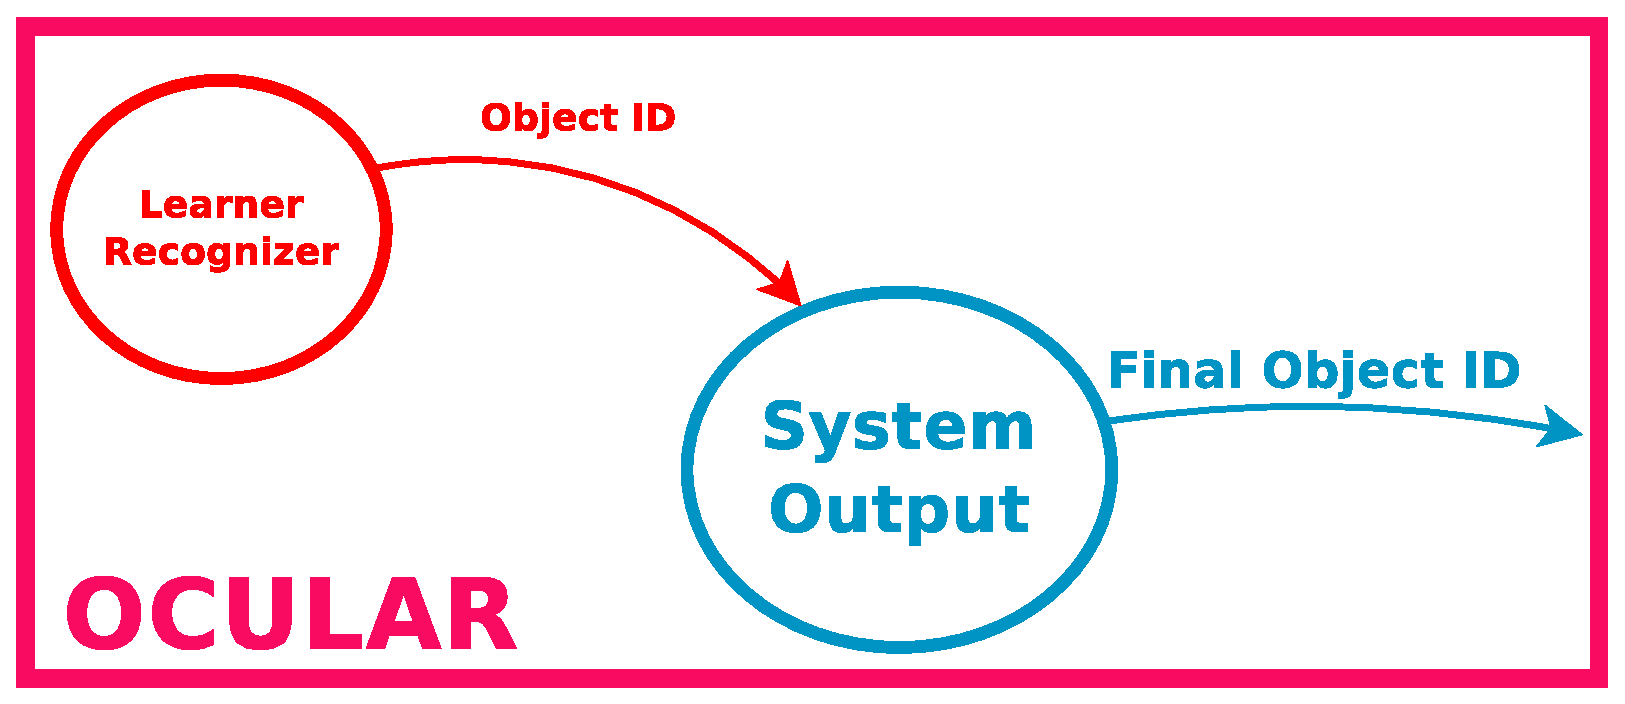
\includegraphics[width=0.5\linewidth]{img/diagrams/node_output.eps}
			\caption[System Output node I/O]{Connectivity graph of the System Output node.}		
			\label{node_output}
			\end{center}
		\end{figure}

	The decision is performed as follows. 
	The thirty 2D and 3D instantaneous object estimations are stored in two vectors. 
	The frequency is the amount of times each object appears in those vectors. 
	This frequency is obtained for 2D and 3D separately.  
	Let us represent as $y'_{2D}$ and $y'_{3D}$ the vectors containing in each element the frequency of the object with $object_id = element$. 
	Both vectors are combined in one, which is called $y'$ using formula \ref{y'}. 
	\begin{center}
	\begin{equation}
	\label{y'}
	y'=0.6*y'_{2D}+0.4*y'_{3D}
	\end{equation}
	\end{center}
	The reason of applying the 0.6 and 0.4 constants for 2D and 3D respectively, instead of calculating a simple mean is because we found empirically that the 2D descriptors produced better predictions than the 3D ones.
	The estimated final object id ($Y$) is obtained as the vector element that has the highest frequency. 
	That is, the final prediction is the object_id whose frequency is higher among the latest 30 predictions.
	This number is $Y$, which is the output of the whole system. 

	\\
	\begin{center}
		$Y'= argmax(y')$
	\end{center} 
	\\
	Figure \ref{uc_output} shows the use case diagram of this node. 

	\begin{figure}[H]
		\centering
			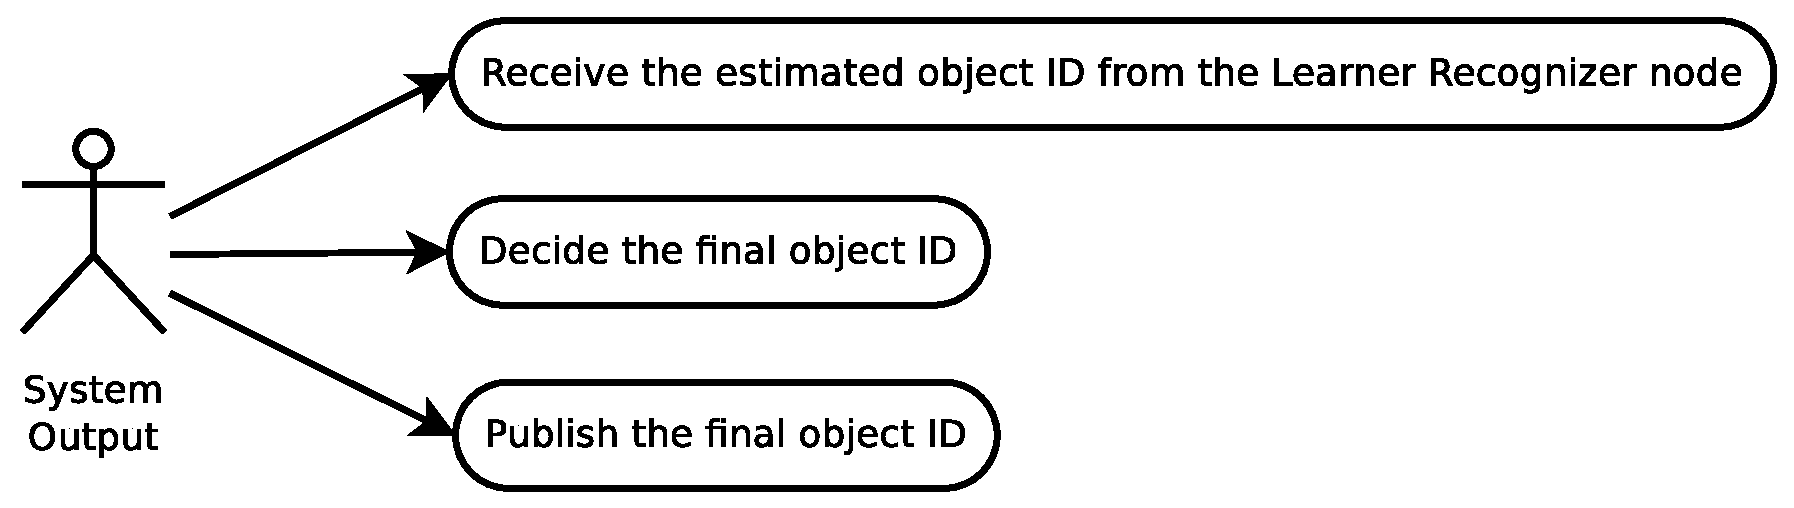
\includegraphics[scale=0.4]{img/diagrams/uc_system_output.eps}
			\caption[Use case diagram System Output node]{Use Case diagram of the System Output node}
			\label{uc_output}
	\end{figure}